\documentclass[11pt,a4paper,twoside,openright]{book}

% 2 added
\usepackage{epsfig}
%\usepackage{epstopdf}

%\usepackage[dvips]{graphicx}
\usepackage{graphicx}
\usepackage{tabularx}
\usepackage[usenames,dvipsnames,svgnames,table]{xcolor}
\usepackage{subfigure}
\usepackage{afterpage}
\usepackage{amsmath,amssymb}
\usepackage{rotating}
\usepackage{fancyhdr}
\usepackage[scriptsize]{caption}

\usepackage{tikz}
\usetikzlibrary{shapes,arrows,matrix,decorations.pathreplacing}

% Define block styles
\tikzstyle{decision} = [diamond, draw, fill=blue!20, 
    text width=5em, text badly centered, node distance=2.3cm, inner sep=0pt]
\tikzstyle{block} = [rectangle, draw, fill=blue!20, 
    text width=8em, text centered, rounded corners, minimum height=2.2em]
\tikzstyle{line} = [draw, -latex']
\tikzstyle{cloud} = [draw, ellipse,fill=red!12, node distance=1.4cm,
    minimum height=2em]

\usepackage{epigraph}
\usepackage{textcomp}
%\usepackage{SIunits}
% 2 added
% \usepackage[colorlinks]{hyperref}
%\usepackage[hidelinks]{hyperref}
\usepackage{lmodern}

%\hypersetup{<option1> [, ...]}
\usepackage{listings}

\definecolor{mygreen}{rgb}{0,0.6,0}
\definecolor{mygray}{rgb}{0.75,0.75,0.75}
\definecolor{mymauve}{rgb}{0.58,0,0.82}


\lstset{
  backgroundcolor=\color{mygray},   % choose the background color; you must add \usepackage{color} or \usepackage{xcolor}
  basicstyle=\tiny,        % the size of the fonts that are used for the code
  breakatwhitespace=false,         % sets if automatic breaks should only happen at whitespace
  breaklines=true,                 % sets automatic line breaking
  captionpos=b,                    % sets the caption-position to bottom
  commentstyle=\color{mygreen},    % comment style
  deletekeywords={...},            % if you want to delete keywords from the given language
  escapeinside={\%*}{*)},          % if you want to add LaTeX within your code
  extendedchars=true,              % lets you use non-ASCII characters; for 8-bits encodings only, does not work with UTF-8
  frame=single,                    % adds a frame around the code
  keepspaces=true,                 % keeps spaces in text, useful for keeping indentation of code (possibly needs columns=flexible)
  keywordstyle=\color{blue},       % keyword style
  language=Matlab,                 % the language of the code
  morekeywords={*,...},            % if you want to add more keywords to the set
  numbers=left,                    % where to put the line-numbers; possible values are (none, left, right)
  numbersep=5pt,                   % how far the line-numbers are from the code
  numberstyle=\tiny\color{mygray}, % the style that is used for the line-numbers
  rulecolor=\color{black},         % if not set, the frame-color may be changed on line-breaks within not-black text (e.g. comments (green here))
  showspaces=false,                % show spaces everywhere adding particular underscores; it overrides 'showstringspaces'
  showstringspaces=false,          % underline spaces within strings only
  showtabs=false,                  % show tabs within strings adding particular underscores
  stringstyle=\color{mymauve},     % string literal style
  tabsize=2,                       % sets default tabsize to 2 spaces
  title=\lstname,                  % show the filename of files included with \lstinputlisting; also try caption instead of title  numbers=left,
  stepnumber=5,
  firstnumber=1,
  numberfirstline=true
}

% \lstset{%
% %  numbers=left,
% %  stepnumber=5,
% %  firstnumber=1,
% %  numberfirstline=true
% 
%   backgroundcolor=\color{mygray},   % choose the background color; you must add \usepackage{color} or \usepackage{xcolor}
%   basicstyle=\footnotesize,        % the size of the fonts that are used for the code
%   breakatwhitespace=false,         % sets if automatic breaks should only happen at whitespace
%   breaklines=true,                 % sets automatic line breaking
%   captionpos=b,                    % sets the caption-position to bottom
%   commentstyle=\color{mygreen},    % comment style
%   deletekeywords={...},            % if you want to delete keywords from the given language
%   escapeinside={\%*}{*)},          % if you want to add LaTeX within your code
%   extendedchars=true,              % lets you use non-ASCII characters; for 8-bits encodings only, does not work with UTF-8
%   frame=single,                    % adds a frame around the code
%   keepspaces=true,                 % keeps spaces in text, useful for keeping indentation of code (possibly needs columns=flexible)
%   keywordstyle=\color{blue},       % keyword style
%   language=Octave,                 % the language of the code
%   morekeywords={*,...},            % if you want to add more keywords to the set
%   numbers=left,                    % where to put the line-numbers; possible values are (none, left, right)
%   numbersep=5pt,                   % how far the line-numbers are from the code
%   numberstyle=\tiny\color{mygray}, % the style that is used for the line-numbers
%   rulecolor=\color{black},         % if not set, the frame-color may be changed on line-breaks within not-black text (e.g. comments (green here))
%   showspaces=false,                % show spaces everywhere adding particular underscores; it overrides 'showstringspaces'
%   showstringspaces=false,          % underline spaces within strings only
%   showtabs=false,                  % show tabs within strings adding particular underscores
%   stepnumber=2,                    % the step between two line-numbers. If it's 1, each line will be numbered
%   stringstyle=\color{mymauve},     % string literal style
%   tabsize=2                        % sets default tabsize to 2 spaces
%   %title=\lstname                   % show the filename of files included with \lstinputlisting; also try caption instead of title
% }

\usepackage{url}

\usepackage{glossaries}
%\hyphenation{a-gen-tiz-za-zio-ne}

\setlength{\paperwidth}{16cm}
\setlength{\paperheight}{24cm}
\setlength{\oddsidemargin} {2. cm}
\setlength{\evensidemargin} {2. cm}
\addtolength{\oddsidemargin} {-0.4 cm}
\addtolength{\evensidemargin} {-0.4 cm}
\linespread{1.1}

% 1 added
\DeclareGraphicsExtensions{.ps,.eps}

% modified
\usepackage[polutonikogreek,english]{babel}
%\usepackage{teubner}
%\usepackage[latin1]{inputenc}

% modified
\usepackage[utf8x]{inputenx}

\renewcommand{\captionfont}{\normalfont \sffamily \itshape \small}

% 1 added
\newcommand{\greek}[1]{{\selectlanguage{polutonikogreek}#1}}

\newcommand{\tikzmark}[1]{\tikz[overlay, remember picture] \coordinate (#1);}

\pagestyle{empty}

%\newcommand{\clearemptydoublepage}{\newpage{\pagestyle{empty}\cleardoublepage}}
\newcommand{\nohyphens}{\hyphenpenalty=10000\exhyphenpenalty=10000\relax}

%% Layout della pagina
%\pagestyle{fancyplain}
%\setlength{\headheight}{14.5pt}
%\addtolength{\headwidth}{\marginparsep}
%\addtolength{\headwidth}{\marginparwidth}
%\renewcommand{\chaptermark}[1]{\markboth{#1}{}}
%\renewcommand{\sectionmark}[1]{\markright{\thesection\  #1}}
%\lhead[\fancyplain{}{\bfseries\thepage}]%
%      {\fancyplain{}{\bfseries\rightmark}}
%\rhead[\fancyplain{}{\bfseries\leftmark}]%
%      {\fancyplain{}{\bfseries\thepage}}
%\cfoot{}

% Questa lunghezza rappresenta la lunghezza completa della pagine, compreso
% lo spazio per le note a margine
%\newlength{\fullpagelen}
%\setlength{\fullpagelen}{\textwidth}
%\addtolength{\fullpagelen}{\marginparsep}
%\addtolength{\fullpagelen}{\marginparwidth}

\makeatletter
\renewenvironment{thebibliography}[1]
  {%
    \chapter*{\bibname}%
    \addcontentsline{toc}{chapter}{\bibname}%
    \@mkboth{\MakeUppercase\bibname}{\MakeUppercase\bibname}%
    \list{\@biblabel{\@arabic\c@enumiv}}%
    {%
      \settowidth\labelwidth{\@biblabel{#1}}%
      \leftmargin\labelwidth
      \advance\leftmargin\labelsep
      \@openbib@code
      \usecounter{enumiv}%
      \let\p@enumiv\@empty
      \renewcommand\theenumiv{\@arabic\c@enumiv}%
    }%
    \sloppy
    \clubpenalty4000
    \@clubpenalty \clubpenalty
    \widowpenalty4000%
    \sfcode`\.\@m%
  }%
  {%
    \def\@noitemerr
    {\@latex@warning{Empty `thebibliography' environment}}%
    \endlist%
  }   % Finisce qui la ridefinizione di thebibliography

\makeatother

 

% \newglossaryentry{naiive}
% {
%   name=na\"{\i}ve,
%   description={is a French loanword (adjective, form of naïf)
%                indicating having or showing a lack of experience,
%                understanding or sophistication},
%   sort=naive
% }


\newacronym{HE}{HE}{Hematoxylin and Eosin}

\newacronym{BC}{BC}{Breast Cancer}

\newacronym{BR}{BR}{Bloom and Richardson Grading System}

\newacronym{NGS}{NGS}{Nottingham Grading System}

\newacronym{HPF}{HPF}{High Power Fields}

\newacronym{CAD}{CAD}{Computer Aided Diagnosis}

\newacronym[longplural=Regions of Interest]{ROI}{ROI}{Region of Interest}

\newacronym{GLCM}{GLCM}{Gray-level Co-occurrence Matrix}

\newacronym{GLEM}{GLEM}{Gray-level Entropy Matrix}

\newacronym{GLRM}{GLRM}{Gray-level Run-length Matrix}

\newacronym{LBP}{LBP}{Local Binary Patterns}

\newacronym{WT}{WT}{Wavelet Transform}

\newacronym{MRI}{MRI}{Magnetic Resonance Imaging}

\newacronym{VAR}{VAR}{Rotation Invariant Variance Measure}

\newacronym{ML}{ML}{Machine Learning}

\newacronym{AI}{AI}{Artificial Intelligence}

\newacronym{TP}{TP}{true positive}

\newacronym{FP}{FP}{false positive}

\newacronym{TN}{TN}{true negative}

\newacronym{FN}{FN}{false negative}

\newacronym{RF}{RF}{Random Forest}

\newacronym{NN}{NN}{Neural Network}

\newacronym{SVM}{SVM}{Support Vector Machine}

\newacronym{CNN}{CNN}{Convolutional Neural Network}

\newacronym{CV}{CV}{Computer Vision}

\newacronym{PR}{PR}{Pattern Recognition}

\newacronym{GGMM}{GGMM}{Gamma Gaussian Mixture Model}

\newacronym{DNN}{DNN}{Deep Neural Network}

\newacronym{ROC}{ROC}{Receiver Operating Characteristic}

\newacronym{RGB}{RGB}{Red-Green-Blue}

\newacronym{HSV}{HSV}{Hue Saturation Value}

\newacronym{RBF}{RBF}{Radial Basis Function}

\newacronym{DT}{DT}{Decision Tree}

\newacronym{PCA}{PCA}{Principal Component Analysis}

\newacronym{GT}{GT}{Ground Truth}

\newacronym{RoR}{RoR}{Ruby on Rails}

\newacronym{CoC}{CoC}{Convention over Configuration}

\newacronym{SVD}{SVD}{Singular Value Decomposition}

% \newglossaryentry{pi}
% {
%   %name={\ensuremath{\pi}},
%   name={pi},
%   description={ratio of circumference of circle to its
%                diameter},
%   sort=pi
% }
% 
% \newglossaryentry{real number}
% {
%   name={real number},
%   description={include both rational numbers, such as $42$ and
%                $\frac{-23}{129}$, and irrational numbers,
%                such as $\pi$ and the square root of two; or,
%                a real number can be given by an infinite decimal
%                representation, such as $2.4871773339\ldots$ where
%                the digits continue in some way; or, the real
%                numbers may be thought of as points on an infinitely
%                long number line},
%   symbol={\ensuremath{\mathbb{R}}}
% }



\makeglossary

\begin{document}

\frontmatter

%%%%%%%%%%%%%%%%%%%%%%%%%%%%%%%FRONTESPIZIO%%%%%%%%%%%%%%%%%%%%%%%%%%%%%%%%%%%

\thispagestyle{empty} \cleardoublepage
\begin{center}
 \LARGE{\textbf{POLITECNICO DI MILANO}}\\
 \mbox{\large{FACOLT\`{A} DI INGEGNERIA DELL'INFORMAZIONE}}\\
 \mbox{\Large{Corso di Laurea Specialistica in Ingegneria Informatica} }
\end{center}

\addvspace{1cm}

\begin{figure}[h]
 \centering
 
\includegraphics[width=3cm]{./images/poli}
\end{figure}

\addvspace{1cm}

\begin{center}
 \begin{large}
  \textbf{MITOSIS DETECTION}
 \end{large}
\end{center}

\addvspace{3cm}
\begin{Large}
 \begin{flushleft}
  \begin{tabbing}
   Relatore: \hspace{8pt}  \= Prof. VINCENZO CAGLIOTI\\
   Correlatore: \> Ing. ALESSANDRO GIUSTI\= \+ \\
  \end{tabbing}
 \end{flushleft}


 \addvspace{3cm}
 \begin{flushright}
 \begin{tabbing}
  %\hspace{240pt}
  \hspace{300pt}
  \= Tesi di laurea di:\\
  \> CLAUDIO G. CACCIA \\
  \> Matr. 751302\\
 \end{tabbing}
 \end{flushright}

 \addvspace{2.5cm}
 \begin{center}
  Anno Accademico 2012 - 2013
 \end{center}

\end{Large}
\newpage
%\clearemptydoublepage


\thispagestyle{empty} \normalfont \cleardoublepage
\vspace{16cm}

%\large
\begin{flushright}
%\itshape{ A Elena, Giovanna e Leonardo}
\itshape{ A ... }
\end{flushright}

\thispagestyle{empty} \cleardoublepage
\pagenumbering{roman}
\newpage
\chapter*{Sommario}

\addcontentsline{toc}{chapter}{Sommario}

%Il sommario deve contenere 3 o 4 frasi tratte dall'introduzione di cui la prima inquadra l'area dove si svolge il lavoro (eventualmente la seconda inquadra la sottoarea pi\`u specifica del lavoro), la seconda o la terza frase dovrebbe iniziare con le parole ``Lo scopo della tesi \`e \dots'' e infine la terza o quarta frase riassume brevemente l'attivit\`a  svolta, i risultati ottenuti ed eventuali valutazioni di questi.

\vspace{1.3cm}
%\noindent NB: se il relatore effettivo \`e interno al Politecnico di Milano nel frontesizo si scrive Relatore, se vi \`e la collaborazione di un altro studioso lo si riporta come Correlatore come sopra. Nel caso il relatore effettivo sia esterno si scrive Relatore esterno e poi bisogna inserire anche il Relatore interno. Nel caso il relatore sia un ricercatore allora il suo Nome COGNOME dovr\`{a} essere preceduto da Ing. oppure Dott., a seconda dei casi.


Il presente lavoro di tesi si colloca nel contesto dell'apprendimento automatico, in particolare 
nel campo della classificazione automatizzata di immagini istologiche.\\
In numerose tipologie di carcinoma, l'identificazione dello stadio di avanzamento della malattia gioca un ruolo fondamentale
per la selezione delle cure migliori e nella riduzione del tasso di mortalit\`{a}. Attualmente, la classificazione
dello stadio di un tumore \`{e} eseguita manualmente dall'istologo su campioni di tessuto analizzati al microscopio.
L'applicazione di tecniche di \textit{computer vision} e di \textit{machine learning} possono portare a numerosi benefici in termini di
tempo e qualit\`{a} delle analisi eseguite.

\vspace{0.3cm}

Il conteggio delle mitosi in un'immagine istologica costituisce uno dei criteri pi\`{u} rigorosi per la classificazione dei tumori e
si rivela essere un'attivit\`{a} complessa anche per un occhio molto allenato. Per tale motivo, l'identifica-zione automatica delle 
mitosi \`{e} un tema di ricerca molto interessante e pu\`{o} essere visto come un caso di apprendimento con supervisione, in cui un classificatore 
ha a disposizione un insieme di immagini di esempio gi\`{a} etichettate e da queste deve inferire dei criteri per classificarne altre.

\vspace{0.3cm}

In generale, da un punto di vista applicativo, l'interesse \`{e} focalizzato sulle prestazioni di un tale sistema: l'obiettivo
consiste nell'ottenere dei risultati uguali o migliori rispetto a quelli ottenuti dall'occhio umano esperto.

\vspace{0.3cm}

In questo lavoro ci poniamo nell'ottica di chi progetta un algoritmo di apprendimento. In questo contesto,
confrontare un algoritmo con un pato-logo esperto non fornisce un'informazione utile: infatti, un medico esperto ha avuto accesso,
durante la sua esperienza lavorativa, ad un insieme di dati di esempio e di linee guida di gran lunga superiori rispetto ad un normale
insieme di \textit{training} di un algoritmo di apprendimento.


\vspace{0.3cm}

Una prestazione inadeguata dell'algoritmo pu\`{o} essere causata dalla sua scarsa capacit\`{a} di identificazione o dalla
mancanza di un numero sufficiente di dati di esempio.
Tramite i risultati delle nostre analisi rispondiamo a tale quesito nel contesto del conteggio di mitosi in immagini istologiche, focalizzandoci sul problema di classificazione.
Abbiamo estratto dei campioni da immagini prese da un \textit{dataset} pubblico e classificato da un patologo esperto.
A questo insieme abbiamo applicato una serie di classificatori ed abbiamo implementato un'interfaccia web per far eseguire 
la classificazione a diversi utenti.

\vspace{0.3cm}

I risultati del confronto dei risultati degli utenti e dei classificatori sviluppati portano alla conclusione che la prestazione degli
algoritmi \`{e} migliore di quella degli umani (risultato coerente con altri studi analizzati) e che quindi la dimensione del dataset
\`{e} un elemento determinante per la determinazione delle prestazioni di un algoritmo di identificazione.

\thispagestyle{empty} \vspace*{.75truecm} \cleardoublepage
\chapter*{Acknowledgements}

\addcontentsline{toc}{chapter}{Acknowledgements}

Ringrazio ................






\tableofcontents


\listoffigures
\addcontentsline{toc}{chapter}{List of Figures}%
\cleardoublepage

\listoftables
\addcontentsline{toc}{chapter}{List of Tables}%
\cleardoublepage

\addcontentsline{toc}{chapter}{Glossary}
\printglossary

\thispagestyle{empty} \vspace*{.75truecm} \normalfont \cleardoublepage
\pagestyle{plain}

\renewcommand{\chaptermark}[1]{\markboth{\chaptername\ \thechapter.\ #1}{}} 
\renewcommand{\sectionmark}[1]{\markright{\thesection.\ #1}}         
\fancyhead[LE,RO]{\bfseries\thepage}    
\fancyhead[RE]{\bfseries\leftmark}    
\fancyhead[LO]{\bfseries\rightmark}     

\renewcommand{\headrulewidth}{0.3pt} 

\mainmatter

\setcounter{page}{1}
\pagenumbering{arabic}

\chapter{Introduction}
\label{Introduction}
\thispagestyle{empty}

\begin{quotation}
{\footnotesize
\noindent{\emph{``Quote 1''}
}
\begin{flushright}
Author 1
\end{flushright}
}
\end{quotation}
\vspace{0.5cm}

%\noindent L'introduzione deve essere atomica, quindi non deve contenere n\`e sottosezioni n\`e paragrafi n\`e altro. Il titolo, il sommario e l'introduzione devono sembrare delle scatole cinesi, nel senso che lette in quest'ordine devono progressivamente svelare informazioni sul contenuto per incatenare l'attenzione del lettore e indurlo a leggere l'opera fino in fondo. L'introduzione deve essere tripartita, non graficamente ma logicamente:


%\section{Inquadramento generale}
%La prima parte contiene una frase che spiega l'area generale dove si svolge il lavoro; una che spiega la sottoarea pi\`u specifica dove si svolge il lavoro e la terza, che dovrebbe cominciare con le seguenti parole ``lo scopo della tesi \`e \dots'', illustra l'obbiettivo del lavoro. Poi vi devono essere una o due frasi che contengano una breve spiegazione di cosa e come \`e stato fatto, delle attivit\`a  sperimentali, dei risultati ottenuti con una valutazione e degli sviluppi futuri. La prima parte deve essere circa una facciata e mezza o due

\emph{First part topics}

\begin{itemize}
\item Detection problems in Computer Vision and in particular in biomedical imaging
\item Relation between detection and classification
\item Mitosis Detection as a component in breast cancer assessment
\item Machine Learning used to automate the mitotic count task
\item The validation problem:
	\begin{itemize}
	\item from clinical point of view
	\item from ML point of view
	\end{itemize}
\end{itemize}

\vspace{0.5cm}

%\section{Inquadramento generale}
%La prima parte contiene una frase che spiega l'area generale dove si svolge il lavoro; una che spiega la sottoarea pi\`u specifica dove si svolge il lavoro e la terza, che dovrebbe cominciare con le seguenti parole ``lo scopo della tesi \`e \dots'', illustra l'obbiettivo del lavoro. Poi vi devono essere una o due frasi che contengano una breve spiegazione di cosa e come \`e stato fatto, delle attivit\`a  sperimentali, dei risultati ottenuti con una valutazione e degli sviluppi futuri. La prima parte deve essere circa una facciata e mezza o due

\emph{Second part topics}

\begin{itemize}
\item General overview of the work: automatic Mitosis Detection in breast cancer histological images and comparison of the performances between humans and algorithms.
	\begin{itemize}
	\item some literature
	\item specificity of this work
	\item achievements
	\item research directions
	\end{itemize}
\end{itemize}


%\section{Breve descrizione del lavoro}
%La seconda parte deve essere una esplosione della prima e deve quindi mostrare in maniera pi\`u esplicita l'area dove si svolge il lavoro, le fonti bibliografiche pi\`u importanti su cui si fonda il lavoro in maniera sintetica (una pagina) evidenziando i lavori in letteratura che presentano attinenza con il lavoro affrontato in modo da mostrare da dove e perch\'e \`e sorta la tematica di studio. Poi si mostrano esplicitamente le realizzazioni, le direttive future di ricerca, quali sono i problemi aperti e quali quelli affrontati e si ripete lo scopo della tesi. Questa parte deve essere piena (ma non grondante come la sezione due) di citazioni bibliografiche e deve essere lunga circa 4 facciate.


\emph{Third part topics}

\begin{itemize}
\item Structure of the work
	\begin{itemize}
	\item Section 1: state of the art...
	\item Section 2: approach to the problem and model
	\item Section 3: design of a mitosis detection algorithm
	\item Section 4: design of a user study
	\item Section 5: experimental results
	\item Section 6: Conclusions
	\item Appendixes: implementation details
	\end{itemize}
\end{itemize}

%\section{Struttura della tesi}
%La terza parte contiene la descrizione della struttura della tesi ed \`e organizzata nel modo seguente.
%``La tesi \`e strutturata nel modo seguente.

%Nella sezione due si mostra \dots

%Nella sez. tre si illustra \dots

%Nella sez. quattro si descrive \dots

%Nelle conclusioni si riassumono gli scopi, le valutazioni di questi e le prospettive future \dots

%Nell'appendice A si riporta \dots (Dopo ogni sezione o appendice ci vuole un punto).''

%I titoli delle sezioni da 2 a M-1 sono indicativi, ma bisogna cercare di mantenere un significato equipollente nel caso si vogliano cambiare. Queste sezioni possono contenere eventuali sottosezioni.

Test riferimenti \cite{SVM01}

\Gls{naiive} people don't know about alternative \gls{computer} operating systems: \glspl{Linux}, BSDs and GNU/Hurd.
\chapter{State of the art}
\label{chapter2}
\thispagestyle{empty}

\begin{quotation}
{\footnotesize
\noindent{\emph{``Rem tene, verba sequentur''}\\
(Know the subject, the words will follow)
}
\begin{flushright}
Marcius Porcius Cato Censorius
\end{flushright}
}
\end{quotation}
\vspace{0.5cm}

%\noindent Nella seconda sezione si riporta lo stato dell'arte del settore, un inquadramento dell'area di ricerca orientato a portare il lettore all'interno della problematica affrontata. Bisogna dimostrare di conoscere le cose fatte fino ad ora in questo campo e il perch\'e si sia reso necessario lo svolgimento di questo lavoro. Questa sezione deve essere grondante di citazioni bibliografiche \cite{Adaptative}.

\section{Background}

\indent \textit{Breast cancer classification} divides breast cancer into categories according to different schemes\footnote{\url{http://www.breastpathology.info/}}, each serving a different purpose.
The purpose of classification is to select the best treatment\cite{Genestie2011}.\\
Within the last decade, histological grading has become widely accepted as a powerful indicator of prognosis in breast cancer. 
The grading depends on the microscopic similarity of breast cancer cells to normal breast tissue, and classifies the cancer as well differentiated (low grade),
moderately differentiated (intermediate grade), and poorly differentiated (high grade), reflecting progressively less normal appearing cells that have a worsening prognosis.
Although grading is fundamentally based on how biopsied, cultured cells behave, in practice the grading of a given cancer is derived by assessing the cellular appearance of the tumor.\\
The \Gls{NGS} (also called Elston-Ellis) is a modification \cite{breastCancerGrading01} of the \Gls{BR}\cite{BRgrading01, BRgenestie}. \Gls{NGS}
is judged more reproducible and is the recommended grading method \cite{NGSrecommended}.


\Gls{NGS} grades breast carcinomas by adding up scores for:\\
\vbox{%
\begin{itemize}
\item tubule formation,
\item nuclear pleomorphism,
\item mitotic count
\end{itemize}}
each of which is given 1 to 3 points. The scores for each of these three criteria and then added together to give an overall final score and corresponding grade as follows \cite{damjanov2007cancer}:\\

\vbox{%
\begin{itemize}
 \item[3-5] \textbf{Grade 1 tumor} (well-differentiated). Best prognosis.
 \item[6-7] \textbf{Grade 2 tumor} (moderately-differentiated). Medium prognosis.
 \item[8-9] \textbf{Grade 3 tumor} (poorly-differentiated). Worst prognosis.
\end{itemize}}

Lower grade tumors, with a more favorable prognosis, can be treated less aggressively, and have a better survival rate.\\

Mitotic activity (see \ref{appendixA} for some details) is one of the strongest prognosticators for invasive breast carcinoma. It is expressed as the number of mitotic figures per tissue area.
Early detection plays an important role in reducing cancer mortality. The current procedure for breast cancer grading is manually performed by pathologists,
for both nuclear pleomorphism \cite{dunne2001scoring} and mitotic count.
Breast tissue samples of patients are taken and examined under microscopes. Pathologists grade the tissue samples based on the deviation of the cell structures
from normal tissues. A pathologist may have to examine a great amount of slides \cite{histopat01}. This process can be time consuming and subjective (see \ref{ch3:humans}).\\
In the following subsection we give a short overview of the mitosis count procedure\cite{amida13}.

\subsection{Tissue preparation}

After tumor excision is performed, the excised material is sent for analysis in a pathology lab.
The tissue preparation process starts with making smaller cuts of the material that are then fixed
in formalin and (after processing) embedded in paraffin.\\
Using a high precision cutting instrument (microtome), thin sections are cut from the
paraffin block, which are then put on glass slides. The final stage of the tissue
preparation process is the staining of the sections with stains that highlight specific
structures of the tissue so they are better visible under a microscope.
The standard staining protocol uses the \Gls{HE} stains.
The hematoxylin dyes the nuclei a dark purple color and the eosin
dyes other structures (cytoplasm, stroma, etc.) a pink color.

\subsection{Digital Pathology}

Recent years have brought the trend of digitization of histological slides. Digital slide
scanners \ref{ch2:fig1}, in combination with digital slide viewers, aim to provide the experience of
viewing a digital slide on a computer monitor in a manner analogous to viewing it under
a microscope, but with all the added benefits of the digital format (ease of annotation,
image analysis, collaborative viewing etc.).
The output of the digital slide scanners are multi-layered images, stored in a format that
enables fast zooming and panning. Depending on the area of the tissue that is present on
the slide and the magnification and resolution at which the slide is scanned, the lowest
layer of the digital slide can be up to several tens of thousands of pixels in width or
height.
Currently, digital slides are mainly used for research, education and remote consultation
purposes. Their use for routine diagnosis and prognosis is not yet common \cite{histopatholImaging01}.
Availability of automatic image analysis algorithms that can aid pathologists in their work can be a major incentive for
acceptance of digital slides in the routine pathology lab workflow.

\begin{figure}[!hbf]
 \begin{center}
  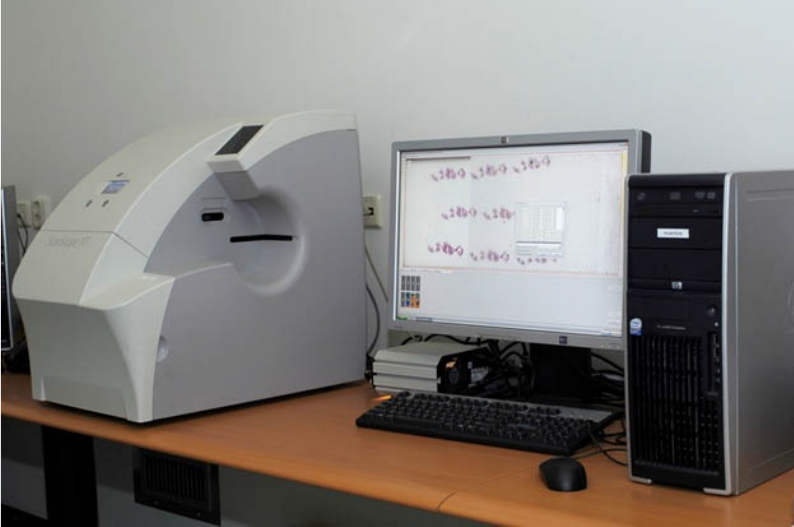
\includegraphics[width=0.6\textwidth]{./images/aperio.png}
  \caption{Aperio ScanScope XT scanner}
  \label{ch2:fig1}
 \end{center}
\end{figure}

\subsection{Mitosis Counting}
Mitotic activity is one of the strongest prognosticators for invasive breast carcinoma and it
is expressed as the number of mitotic figures per tissue area. As part of the \Gls{BR} grading system, mitotic activity is
routinely assessed in pathology labs across the world. In addition, the mitotic activity
can be used as a prognosticator independently of the \Gls{BR} grading system.
Typically, the pathologist receives a panel of slides for each case that is to be graded. He
or she then proceeds to select one slide where the histological grading will be
performed. The mitosis counting is performed in 8-10 consecutive microscope \Gls{HPF} \cite{breastCancerMitosisPCA_ICA}. 
A HPF has a size of $512 \times 512 \mu m^{2}$ (i.e. an area of 0.262 $mm^{2}$ ), which is the equivalent of a microscope field diameter of $0.58mm$.
The standard guidelines are to select an area that encompasses the most invasive
part of the tumor, at the periphery and with highest cellularity. Depending on the
number of figures counted, a mitotic activity score is assigned. Cases with 7 or fewer
mitotic figures present are assigned score 1 (best prognosis). Cases with more than 12
mitotic figures are assigned score 3 (worst prognosis). The intermediate cases are
assigned score 2.

\subsection{Challenges in Mitosis Detection}
Because of the aberrant chromosomal makeup of many tumors (aneusomy, polysomy,
translocations, amplifications, deletions), the appearance of mitotic figures in the
images can significantly differ from the textbook examples of a splitting nucleus\cite{mitosisDetectBreastCancer01}. In
addition, imperfections of the tissue preparation process result in tissue appearance
variability, which can present a challenge also for an automated mitosis detection system.\\
Most commonly, mitotic figures are exhibited as hyperchromatic objects. In addition,
they have absence of a clear nuclear membrane, \textquotedblleft hairy\textquotedblright protrusions around the edges
and basophilia instead of eosinophilia of the surrounding cytoplasm. However, these are
more guidelines than hard rules, and the bulk of the training of pathologists is done by
looking as specific examples of mitotic figures.
One of the main challenges in spotting mitotic figures is that other objects such as
apoptotic nuclei can have similar appearance, making it
difficult even for trained experts to make a distinction \cite{mitosisDetectionLearningBased}. Lymphocytes, compressed
nuclei, \textquotedblleft junk\textquotedblright particles and other artifact form the tissue preparation process, can also
have hyperchromatic appearance.
The images in Figure \ref{ch2:fig2} and in Figure \ref{ch2:fig3} try to give an idea of the difficulty of the task.

\begin{figure}[!hbt]
  \centering
    \subfigure[]{
      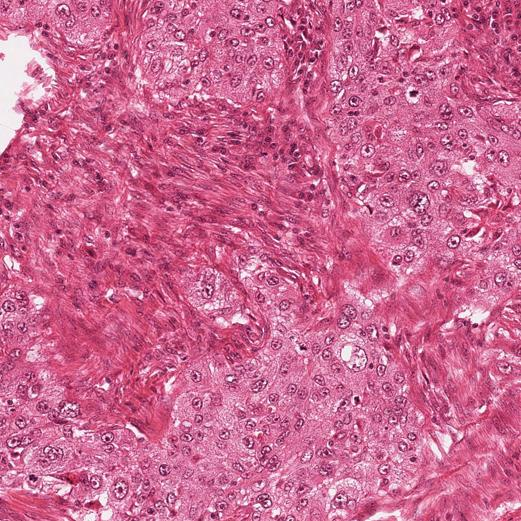
\includegraphics[width=0.44\textwidth]{./images/A00_06th.jpg}
      \label{ch2:fig2:a}
    }
    \hspace{2mm}
    \subfigure[]{
      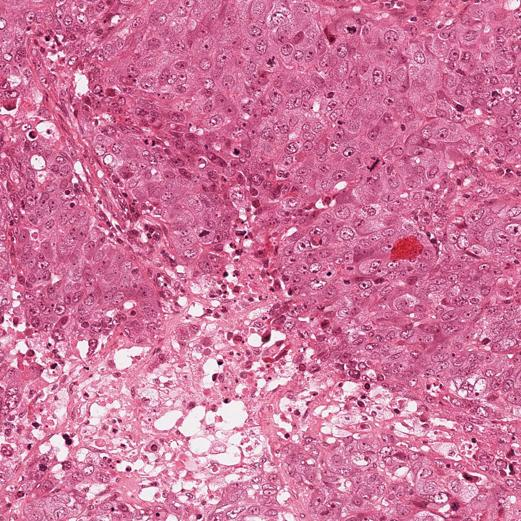
\includegraphics[width=0.44\textwidth]{./images/A01_05th.jpg}
      \label{ch2:fig2:b}
    }\\
    \vspace{2mm}
    \subfigure[]{
      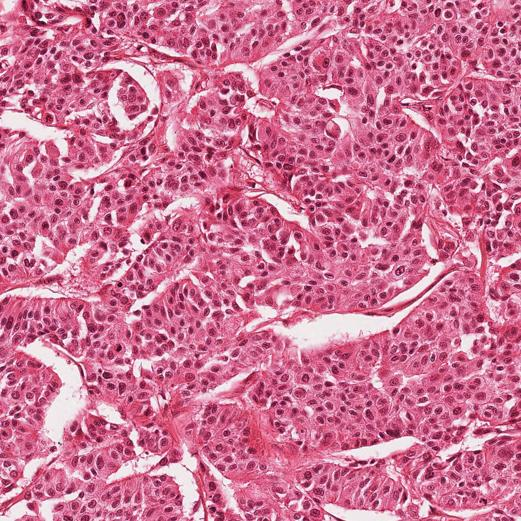
\includegraphics[width=0.44\textwidth]{./images/A02_02th.jpg}
      \label{ch2:fig2:c}
    }
    \hspace{2mm}
    \subfigure[]{
      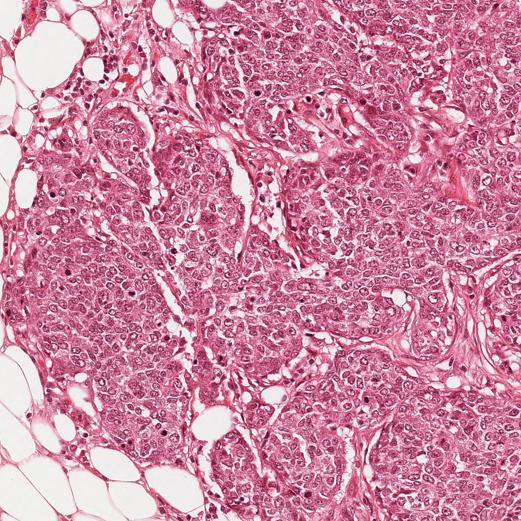
\includegraphics[width=0.44\textwidth]{./images/A03_02th.jpg}
      \label{ch2:fig2:d}
    }
    \caption{Examples of digital histological images}
    \label{ch2:fig2}
\end{figure}

\vspace{0.5cm}

\section{Mitosis Detection and Computer Vision}


The task of automatic mitosis detection involves topics in varius fields of research, in particular

\begin{itemize}
 \item Image Analysis
 \item Machine Learning
\end{itemize}

We consider a framework in which, in the whole image, some candidates are detected and the classified as mitosis or non-mitosis.\\
In this chapter we give an overview of the main aspects concerning \textit{image analysis} and in the following one (\ref{ch2:ML}) we analyze the \textit{machine learning} elements.




\subsection{Overview of Medical Imaging}

Over the past decade, dramatic increases in computational power and improvement in image analysis algorithms have
allowed the development of powerful computer-assisted analytical approaches to radiological and histo-pathological data\cite{HistopatImaging01Review}.
Digitized tissue histopathology has now become ame-nable to the application of computerized image analysis and machine learning techniques.
Analogous to the role of \Gls{CAD} algorithms in medical imaging to complement the opinion of a radiologist, \Gls{CAD} algorithms have begun to be developed for
disease detection, diagnosis, and prognosis prediction to complement the opinion of the pathologist\cite{sertel2009computer}.

\subsection{Software Tools}

The imaging modalities rely heavily on computational approaches. In fact, in many cases the computational technology is just as important as the optics,
not just for the digital capture that all systems now use but in many cases also for visualizing and properly interpreting the data.
The article in 	\cite{BioImagingSW05} reviews each computational step that biologists encounter when dealing with digital images and the overall status of available software for bioimage informatics.
It is worth highlighting the existence of open-source software tools like \textit{Fiji} \cite{BioImagingSW03} and \textit{ImageJ} \cite{BioImagingSW02}, which supply some basic features
for \textit{object detection} and \textit{feature extraction}\cite{featuresReviewBioinformatics}.

\vspace{0.5cm}


\subsection{Features}

The concept of feature is used to denote a piece of information which is relevant for solving a computational task\cite{featExtractionAndImageProcessingBook}.
A feature is defined as an \textquotedblleft{interesting}\textquotedblright part of an image, and features are used as a starting point for many computer vision algorithms.
They can be the result of a general \textit{neighborhood operation}\cite{jahne2000computer} applied to the image, or specific structures in the image itself.
Types of image features include:
\begin{itemize}
 \item Edges
 \item Corners
 \item Blobs or \Glspl{ROI}
 \item Ridges or elongated objects (i.e. blood vessels in medical images)
\end{itemize}

Other examples of features are related to motion in image sequences, to shapes defined in terms
of curves or boundaries between different image regions, or to properties of such a region\cite{MVG_Hartley2004}.

The feature concept is very general and the choice of features in a particular computer vision system may be highly dependent on the specific problem to be considered.\\


\subsection{Feature Detectors}

Many algorithms have been developed to detect specific features, and a complete overview of them is beyond
the scope of this work. Some of the most famous ones, like \textit{Canny edge detector}\cite{canny},
\textit{Harris edge and corner detector}, or SUSAN \cite{detectSusan} are available in most widely used
commercial and open-source Computer Vision software packages (i.e. {\scshape Matlab}
Image Processing Toolbox\footnote{\url{http://www.mathworks.com/products/image/index.html}} or OpenCV\footnote{\url{http://opencv.org/}} ).\\

Features are sometimes extracted over several scalings. One of these methods is \textit{Scale-invariant feature transform};
in this algorithm, various scales of the image are analyzed to extract features\cite{LoweScale} (the underlying theory can be found in \cite{feature01ScaleSpace}).\\


\subsection{Image Segmentation}
\label{ch2:IS}
Segmentation is the process of partitioning a digital image into multiple segments (sets of pixels) in order to simplify
or change the representation of an image into something that is more meaningful and easier to analyze\cite{breastCancer02}.
Image segmentation is typically used to locate objects and boundaries (i.e. features) in images. 
Such a process assigns a label to every pixel in an image so that pixels with the same label share certain visual characteristics\cite{mitosisDetectionLearningBased}.


\subsection{Texture Algorithms}

An image texture is a set of metrics designed to quantify the perceived texture of an image.
Image texture gives information about the spatial arrangement of color or intensities in an image or in selected region of it\cite{ CV_Forsyth}.
Image textures are used in \textit{segmentation}(see \ref{ch2:IS}), or \textit{classification} of images (see \ref{ch2:ML}).
To address the issue of texture analysis, the so called \textquotedblleft{}statistical approach\textquotedblright  is more widely used as it is easier to compute.
This approach sees an image texture as a quantitative measure of the arrangement of intensities in a region.

\subsubsection{Co-occurrence Matrix}

Co-occurrence matrix captures numerical features of a texture using spatial relations of similar gray tones.
Numerical features computed from the co-occurrence matrix can be used to represent, compare, and classify textures\cite{textureGLCMexample, textureGLCM_wood}.
The following are a subset of standard features derivable from a normalized co-occurrence matrix, as described in \cite{haralick1973textural}:

\begin{eqnarray}
\textrm{Contrast} & = & \sum_{n=0}^{N_g-1} n^{2} \left\{ \sum_{i=1}^{N_g} \sum_{j=1}^{N_g} p[i,j] \right\}, \ \textrm{where} |i-j| = n \\
\textrm{Correlation} & = & \frac{ \sum_{i=1}^{N_g} \sum_{j=1}^{N_g} (i,j) \cdot p[i,j] - \mu_x \mu_y }{\sigma_x \sigma_y} \\
\textrm{Entropy} & = & - \sum_{i} \sum_{j} p[i,j] \cdot \log(p[i,j])
\end{eqnarray}

Where:
\begin{itemize}
 \item $N_g$ is the number of gray levels in the quantized image,
 \item $p[i,j]$ is the $(i,j)th$ entry in a normalized gray-tone spatial dependence matrix,
 \item $\mu_x,\sigma_x,\mu_y,\sigma_y$ are the mean and the standard deviation of respectively $p_x = \sum_{j=1}^{N_g}p(i,j)$ and  $p_y = \sum_{i=1}^{N_g}p(i,j)$.
\end{itemize}

Various algorithms use texture feature like \Gls{GLCM} \cite{texture03}, \Gls{GLRM} \cite{texture02} or \Gls{GLEM} for image classification,
also in medical \cite{texture04} and biological imaging \cite{textGLCMbiol}.


\subsubsection{Local Binary Patterns}

\Gls{LBP} is another type of feature used for classification in computer vision. \Gls{LBP} is a simple yet very efficient texture operator
which labels the pixels of an image by thresholding the neighborhood of each pixel with the value of the center pixel and considers the result as a binary number.
The distance and the number of neighbors can be selected, as shown in Figure \ref{ch2:fig4}\cite{LBP01}.
The notation $(P,R)$ is used for pixel neighborhoods which means \textit{P} sampling points on a circle of radius of \textit{R}.

\begin{figure}[!htb]
  \centering
    \subfigure[(8,1)]{
      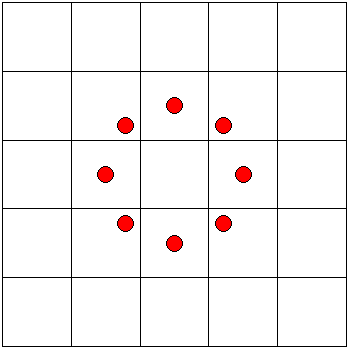
\includegraphics[width=0.25\textwidth]{./images/lbp1_c.png}
      \label{ch2:fig4:a}
    }
    \hspace{1mm}
    \subfigure[(8,2)]{
      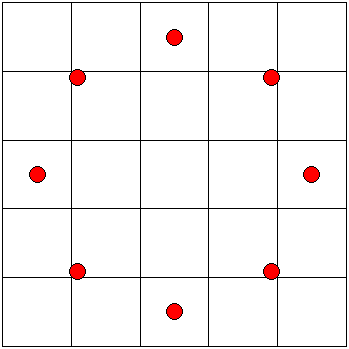
\includegraphics[width=0.25\textwidth]{./images/lbp2_c.png}
      \label{ch2:fig4:b}
    }
    \hspace{1mm}
    \subfigure[(16,3)]{
      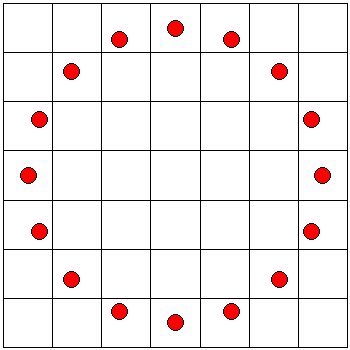
\includegraphics[width=0.25\textwidth]{./images/lbp3_c.png}
      \label{ch2:fig4:c}
    }    
    \caption{Examples LBP neighbors and distances}
    \label{ch2:fig4}
\end{figure}

The computation of the \Gls{LBP} code of a pixel of coordinates $(x_c,y_c)$ is given by:

\begin{equation}
 LBP_{P,R} = \sum_{p=0}^{P-1} s(g_p - g_c) \cdot 2^{p} \quad \textrm{where} \ s(x) = 
    \left\{
	\begin{array}{ll} 1, & \textrm{if} \ x \geq 0\\
			  0, & \textrm{otherwise}
	\end{array}
    \right.
\end{equation}

This operator used jointly with a simple local contrast measure provided very good performance in unsupervised texture segmentation.
Another extension to the original operator is the definition of so called uniform patterns, which can be used to reduce the length of the feature
vector and implement a simple rotation-invariant descriptor. This extension was inspired by the fact that some binary patterns occur more commonly
in texture images than others. A \Gls{LBP} is called uniform if the binary pattern contains at most two bitwise transitions from 0 to 1
or vice versa when the bit pattern is traversed circularly.\\
. In the computation of the \Gls{LBP} labels, uniform patterns are used so that there is a separate label for each uniform pattern and all
the non-uniform patterns are labeled with a single label.
For example, when using $(8,R)$ neighborhood, there are a total of 256 patterns, 58 of which are uniform, which yields in 59 different labels. 

The uniform and rotation invariant \Gls{LBP}  can be further enhanced by combining it with a \Gls{VAR} operator, with the same parameters $(P,R)$,
that characterizes the contrast of local image texture\cite{LBP02}.
Both operators are also computationally attractive, as they can be realized with a few operations in a small neighborhood and a lookup table.
The \Gls{VAR} operator is described by the following relations:

\begin{equation}
 VAR_{(P,R)} = \frac{1}{P} \sum_{p=0}^{P-1}(g_p - \mu)^{2} \quad \textrm{where} \ \mu = \sum_{p=0}^{P-1}g_p^2
\end{equation}

\Gls{LBP}$(P,R)$ and \Gls{VAR}$(P,R)$ are complementary and a feature set made by the combination of the two is expected to be a very
powerful rotation invariant measure of local image texture. It is also possible to use joint feature sets composed by operators with different neighborhood.

\subsubsection{Wavelets}

The \Gls{WT} is having greater importance medicine and biology.
The main uses of the \Gls{WT} concern the analysis of one-dimensional physiological signals obtained by electrocardiography (ECG)
and electroencephalography (EEG), including evoked response potentials\cite{wavelets}.
A survey of recent wavelet developments in medical imaging can be found in \cite{waveletsBiomed}.
These include biomedical image processing algorithms (e.g., noise reduction, image enhancement, and detection) and
image reconstruction and acquisition schemes (tomography, and \Gls{MRI}).


\subsection{Object detection and recognition}

Object detection is a computer vision technology that deals with detecting instances of semantic objects of a certain class (such as humans, traffic signs, mitotic cells) in digital images
Humans recognize a multitude of objects in images with little effort, despite the fact that the image of the objects may be in different orientation,
or in different size/scale. Objects can even be recognized when they are partially obstructed from view.
This task is still a challenge for computer vision systems and represents the connection between Image Analysis topics and Machine Learning.
Viola and Jones proposed a well known object detection framework \cite{objDetect04ViolaJones, objDetect05ViolaJonesRapid}, which involves the sums
of image pixels within rectangular areas, using the so-called Haar-like features, a name that resembles the Haar wavelet adopted in \cite{objDetect03framework}.
The technique generates a large amount of features and uses the boosting algorithm \textit{AdaBoost} to reduce the over-complete set, by selecting the best features and training classifiers that use them.
The evaluation of the classifiers generated in the learning phase can be quick, but generally not enough to be run in real-time. For this reason, the classifiers are arranged in a cascade in order of complexity,
where each susequent classifier is trained only on those selected samples which pass through the preceding classifiers.
If at any stage in the cascade a classifier rejects a sample, no further processing is performed.
The cascade therefore has the form of a degenerate tree.


\vspace{0.5cm}

\begin{figure}[!hbt]
 \centering
  \subfigure[source image]{
    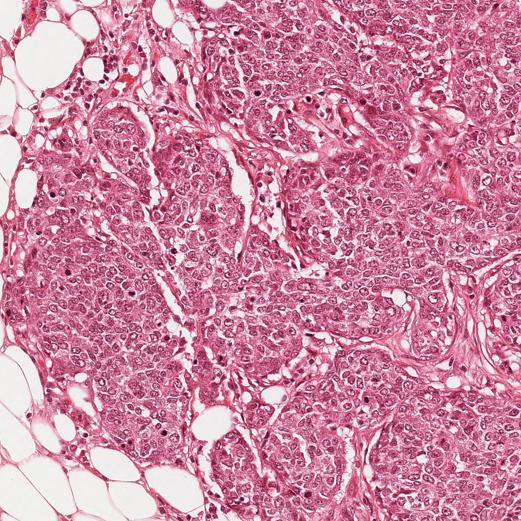
\includegraphics[width=0.72\textwidth]{./images/A03_02th.jpg}
    \label{ch2:fig3:a}
   }\\
  \subfigure[mitoses]{
    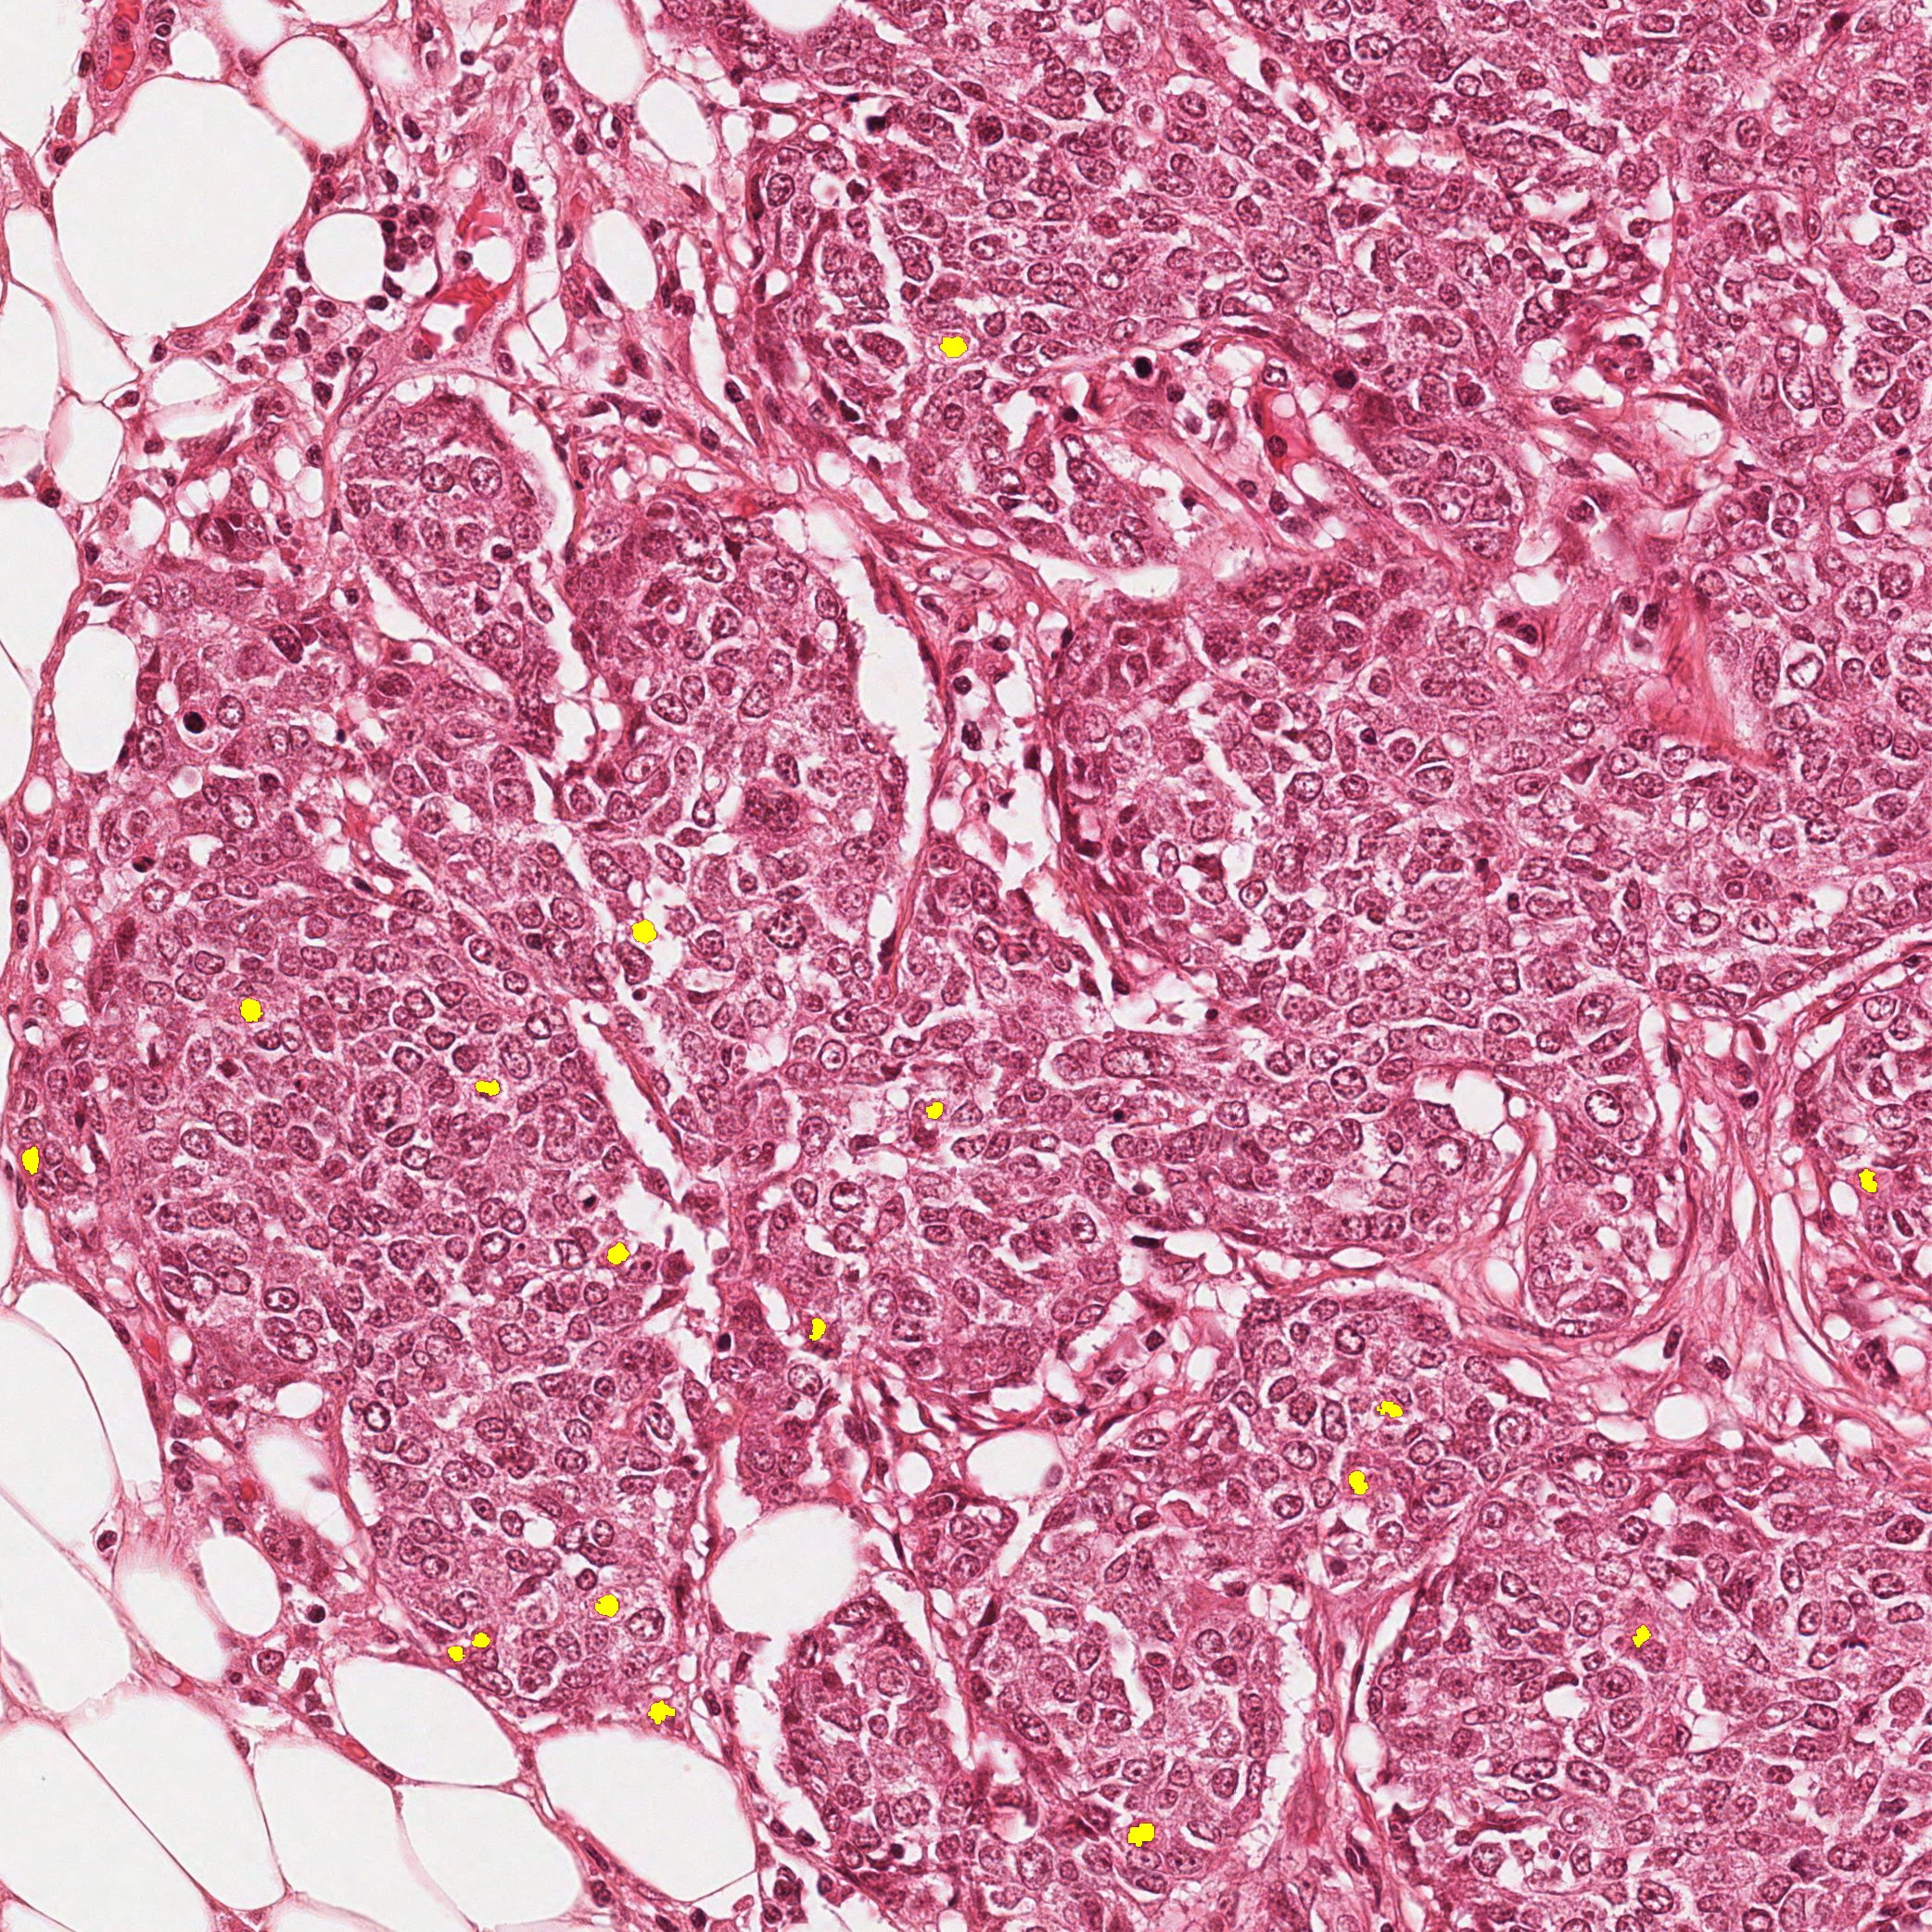
\includegraphics[width=0.72\textwidth]{./images/A03_02.jpg}
    \label{ch2:fig3:b}
  }
  \caption{Example of image with highlighted mitoses (yellow) }
  \label{ch2:fig3}
\end{figure}


\section{Machine Learning}
\label{ch2:ML}

\Gls{ML}, a branch of \Gls{AI}, deals with the ability to define and to build systems that can learn from data.
The core of \Gls{ML} deals with the representation of data and their generalization. Representation deals with the way the system describes the data.
Generalization deals with the ability of the system to perform on unseen data samples.
In Machine Learning, the observations are often known as \textit{instances},
the explanatory variables are termed \textit{features} (grouped into a \textit{feature vector}), and the possible categories to be predicted are \textit{classes}. 


\Gls{ML} algorithms can be divided into different types:
\begin{itemize} 
 \item [-] \textbf{Supervised Learning} generates a function that maps inputs to desired outputs usually called \textit{labels},
	because they are often provided by human experts classifying the training examples.
 \item [-] \textbf{Unsupervised learning} models a set of inputs. It can also be referred to as \textit{data mining} and knowledge discovery. Here, labels are not known during training.
 \item [-] \textbf{Semi-supervised learning} combines both labeled and unlabeled examples to generate an appropriate function or classifier. 
 \item [-] \textbf{Reinforcement learning} learns how to act given an observation of the world. Every action has some impact in the environment, and the environment provides feedback in the form of rewards that guides the learning algorithm.
\end{itemize}

There exists a great variety of \Gls{ML} algorithms, and a detailed review is beyond the scope of this work\footnote{A list of \Gls{ML} algorithms can be found in
\url{http://en.wikipedia.org/wiki/List_of_machine_learning_algorithms}}.\\
We focous, in our analysis, on \textit{Pattern Recognition} and in particular on \textit{Supervised Learning} methods.

\subsection{Pattern Recognition}

Pattern recognition is the assignment of a label to a given input value \cite{bishop2006pattern, theodoridis2008pattern}. In its most general form, pattern recognition involves:

\begin{itemize}
 \item \textbf{Classification} is the problem of identifying to which of a set of categories a new observation belongs, on the basis
 of a training set of data containing instances whose category membership is known,
 \item \textbf{Regression} is a technique for estimating the relationships among variables, assigning a real-valued output to each input,
 \item \textbf{Sequence labeling} refers to the assignment of a categorical label to each member of a sequence of observed values,
 in particular by making choices which depend on the one made for nearby elements (e.g. speech tagging)
 \item \textbf{Parsing} is the process of analyzing a string of symbols according to the rules of a formal grammar.
\end{itemize}

\subsection{Classification}

Among the different types of learning methods and pattern recognition techniques we focus our attention on \textit{classification} which, in general \Gls{ML} 
terminology, is an instance of \textit{supervised learning}.\\
The formal definition of a supervised classification problem can be stated as follows: an unknown function $g$ maps the input instances $x \in X$ to the output labels $y \in Y$:

\begin{equation}
 \label{ch2:eq1}
 g: X \rightarrow Y
\end{equation}

Equation \ref{ch2:eq1} represents the \textit{ground truth}.\\
The \textit{training set}
\begin{equation}
 T = { (x_1,y_1), \ldots ,(x_n,y_n) }
\end{equation}

is assumed to represent the mapping of $g$ in an accurate way. The classifier then tries to build a function $h: X \rightarrow Y$ that approximates as closely as possible the correct mapping. The measure of the performance
(see \ref{ch3:Bench} for details) is generally done on a separate set of data ( the \textit{test set}) whose labels are known but whose data are not used during the learning phase\cite{liu2006pattern}.

A common subclass of classification is \textit{probabilistic classification}. Algorithms of this type involve statistical tools to define the best class for a given instance\cite{ML_gaussian}.
Probabilistic algorithms output a probability that the instance is a member of each of the possible classes. The best class is normally then selected as the one with the highest probability.
Classification can be also divided into two separate problems - \textit{binary classification} and \textit{multi-class classification}.
In binary classification, only two classes are involved, whereas multi-class classification considers the problem of assigning an object to one of several classes.
Since many classification methods have been developed specifically for binary classification, multi-class classification often requires the combined use of multiple binary classifiers.

\subsection{Binary Classification}

Binary classification is the task of classifying the members of a given set of objects into two groups on the basis of whether they have some property or not\cite{scholkopf2002learning}.
Medical testing is a typical binary classification task (i.e. to determine if a patient has certain disease or not ).
In traditional statistical hypothesis testing, the tester starts with a null hypothesis and an alternative hypothesis,
performs an experiment, and then decides whether to reject the null hypothesis in favor of the alternative.
Hypothesis testing is therefore a binary classification of the hypothesis under study \cite{mitchML}.
A \textit{positive} result is one which rejects the null hypothesis.
Rejecting the null hypothesis when it is actually true - a \Gls{FP} - is a \textbf{type I error};
on the other hand, when the null hypothesis is false results in a \Gls{TP}.
A \textit{negative} result is one which does not reject the null hypothesis.
Accepting the null hypothesis when it is actually false - a \Gls{FN} - is a \textbf{type II error};
on the other hand, when the null hypothesis is true results in a \Gls{TN}.
How the number of \Gls{TP}, \Gls{FP}, \Gls{TN} and \Gls{FN} can be used to assess the performances of a classification algorithm is treated in Section \ref{ch3:Bench}.


\subsection{Binary Classifiers}

An algorithm that implements a classification, is defined a \textbf{classifier}.
The term also refers to the mathematical function, implemented by a classification algorithm, that maps input data to a category (i.e. \textit{class}).
A great amount of algorithms has been developed for classification purposes, in particular for computer vision tasks \cite{classificationSurvey}.
Some methods suitable for learning binary classifiers include\cite{dataMiningBook}:

\begin{itemize}
 \item Naive Bayes classifiers
 \item Bayesian networks \ \cite{bayesClassifiersCellSegmentation}
 \item Decision trees \ \cite{randTree01}
 \item \Glspl{RF} \ \cite{randForests01}
 \item \Glspl{SVM} \ \cite{SVM01}
 \item Hidden Markov models
 \item \Glspl{NN} \ \cite{russell2010artificial}
\end{itemize}


In our work we focused on two types of classifiers: \textit{Support Vector Machines} and \textit{Random Forests}
which are widely used in computer vision classification problems ( e.g. \cite{mitosisDetectionLearningBased} and \cite{randForests04}).

\subsection{Software Tools}

Classification tasks can be accomplished by a large amount of software tools. Here we mention the ones that we consider to be the most relevant ones.\\
\textit{Weka} \cite{dataMining_Weka, dataMining_Weka_upd} is a \textbf{FLOSS} general purpose data mining software tool developed by the Waikato University
\footnote{\url{http://www.cs.waikato.ac.nz/ml/weka/}} which allows to implement a great variety of classifiers \cite{dataMiningBook}. It also has an interface
with \textbf{R} \footnote{\url{http://cran.r-project.org/}} \cite{hornik2009open}.\\
{\scshape Matlab} can perform classification task by means of some of its toolboxes (i.e. Bioinformatics \footnote{\url{http://www.mathworks.com/products/bioinfo/} }
and Statistics \footnote{\url{http://www.mathworks.com/products/statistics/} } ).


\vspace{0.5cm}


\chapter{Problem Definition}
\label{chapter3}
\thispagestyle{empty}

\begin{quotation}
{\footnotesize
\noindent{\emph{``\greek{p'antec >'anjrwpoi to~u e>id'enai >or'egontai f'usei}''}\\
(All men naturally desire knowledge)}
\begin{flushright}
\greek{>Aristot'elhc}(Aristotle, Met. 1.980a)
\end{flushright}
}
\end{quotation}


%\noindent In questa sezione si deve descrivere l'obiettivo della ricerca, le problematiche affrontate ed eventuali definizioni preliminari nel caso la tesi sia di carattere teorico.


\section{Bacground}

The purpose of automating the mitosis detection problems requires the definition 

\begin{tikzpicture}[node distance = 2cm, auto]
    % Place nodes
    \node [block] (init) {initialize model};
    \node [cloud, left of=init] (expert) {expert};
    \node [cloud, right of=init] (system) {system};
    \node [block, below of=init] (identify) {identify candidate models};
    \node [block, below of=identify] (evaluate) {evaluate candidate models};
    \node [block, left of=evaluate, node distance=3cm] (update) {update model};
    \node [decision, below of=evaluate] (decide) {is best candidate better?};
    \node [block, below of=decide, node distance=3cm] (stop) {stop};
    % Draw edges
    \path [line] (init) -- (identify);
    \path [line] (identify) -- (evaluate);
    \path [line] (evaluate) -- (decide);
    \path [line] (decide) -| node [near start] {yes} (update);
    \path [line] (update) |- (identify);
    \path [line] (decide) -- node {no}(stop);
    \path [line,dashed] (expert) -- (init);
    \path [line,dashed] (system) -- (init);
    \path [line,dashed] (system) |- (evaluate);
\end{tikzpicture}












\vspace{0.5cm}



\section{From Detection to Classification}

The process of detection and classification....

\vspace{0.5cm}

\section{Definition of Classification}

Definition of classification:
\begin{itemize}
\item input
\item output
\item classes
\end{itemize}

\vspace{0.5cm}

\section{Classification Assessment}

\subsection{Algorithms}






In our work we focused on two types of classifiers: \textit{Support Vector Machines} and \textit{Random Forests}
which are widely used in computer vision classification problems ( e.g. \cite{mitosisDetectionLearningBased} and \cite{randForests04}).
We also mention \Glspl{CNN} because they played a relevant role in the definition of our dataset [REF].


 

The role of features and classifiers

\subsection{Feature Extraction}

Curse of dimensionality and PCA










[SNIPPET]
In most computer vision applications it is not sufficient to extract only one type of feature to obtain the relevant information from the image data.
Instead two or more different features are extracted, resulting in two or more feature descriptors at each image point.
A common practice is to organize the information provided by all these descriptors as the elements of one single vector,
commonly referred to as a feature vector. The set of all possible feature vectors constitutes a feature space.
A common example of feature vectors appears when each image point is to be classified as belonging to a specific class.
Assuming that each image point has a corresponding feature vector based on a suitable set of features,
meaning that each class is well separated in the corresponding feature space, the classification of each image point can be done using standard classification method.






\subsection{Humans}

Experience, agreement...

\vspace{0.5cm}

\section{Performance}

Definition of performance


[SNIPPET]
The general appearance of a mitosis results in the fact that automatically detecting mitoses is very challenging.
Different to other pattern recognition tasks, mitotic cells essentially are irregular shape objects. As a result, there
is no simple way of extracting the features of mitotic cells.
Benchmarking of different detection algorithms and comparison with human performance.


\section{Benchmarks}
\label{ch3:Bench}

\vspace{0.5cm}

\subsection{Humans}
\label{ch3:humans}


Agreement between different histologists

\subsection{Algorithms}

The technique of \textit{thresholding} is often used to analyze the performance of an algorithm that outputs probabilities in 


\chapter{Design of a Mitosis Detection algorithm}
\label{chapter4}
\thispagestyle{empty}

\begin{quotation}
{\footnotesize
\noindent \emph{\textquotedblleft Ab uno\\ disces omnis\textquotedblright}\\
\noindent (Learn everything from one)
\begin{flushright}
Publius Vergilius Maro (Aeneis II, 65-66)
\end{flushright}
}
\end{quotation}

\vspace{2cm}

%\noindent In questa sezione si spiega come \`e stato affrontato il problema concettualmente, la soluzione logica che ne \`e seguita senza la documentazione.

We developed an algorithm to perform mitosis-detection as a part of our work, with the aim to compare its results with humans facing the same task.

\section{Dataset}
\label{ch4:ds}

We used the public MITOS dataset \cite{icpr}. The dataset is composed by a total of 50 images with size 2084$\times$2084 pixel,
covering an area of 512$\times$512 $\mu$m each, acquired with an APERIO XT scanner (see Figure \ref{ch2:fig1}). 
A unique split is defined by the dataset authors, with 35 images used for training and 15 for evaluation.
The dataset contains a total of about 300 mitosis, which were annotated by an expert pathologist.
The performance of the algorithms participating to the \textit{2012 ICPR mitosis detection contest} are shown in Section \ref{ch3:icpr_perf}.\\
With reference to Figure \ref{ch3:fig1}, we focused on on the classification subproblem, with the \Glspl{ROI} given as an input.
The input is given in form of an image patch with size 100$\times$100 pixel: such size completely contains the image of the cell.
\clearpage
\noindent The task is to map each patch to one of two classes:
\begin{itemize}
 \item [] \textit{\textbf{C1}}: the image contains a mitosis at its center,
 \item [] \textit{\textbf{C0}}: the image does not contain a mitosis anywhere. 
\end{itemize}

\noindent There are no samples in which a mitosis is visible off-center.

\vspace{0.5cm}

\subsection{Image Candidates}
\label{ch4:ic}

For the \textit{\textbf{C1}} class, all the 216 mitosis available in the 35 training images are chosen
as training samples, and all 87 mitosis in the evaluation images are chosen as
evaluation samples.\\
We enforced an even distribution of the two classes classes both in training and in evaluation sets, and therefore
selected 216 \textit{\textbf{C0}} samples for training and 87 \textit{\textbf{C0}} samples for evaluation; the resulting
training set contained 432 samples.\\
Millions of different \textit{\textbf{C0}} samples may be randomly chosen from the original training and evaluation images:
an overwhelming majority of such samples would not contain any nucleus and therefore be non-informative for training and trivial for
evaluation. Limiting the choice to non-mitotic nuclei \texttwelveudash{} which greatly outnumber
mitotic ones \texttwelveudash{} would not solve the problem, since most of such nuclei look very
similar to each other and are trivially identified as non-mitotic. Only a small
subset of non-mitotic nuclei \texttwelveudash{} as well as other structures and artifacts \texttwelveudash{} pose an
actual challenge, both for humans and for algorithms.\\
In order to select such objects as \textit{\textbf{C0}} samples, we used the output produced by a simple \Gls{CNN}-based mitosis detector,
similar to the one outlined in another work on the same dataset \cite{agNN}, for selecting useful training samples.
The detector, built at IDSIA, was trained on few images in the training set, then applied on the whole dataset.
Because the detector was simple and trained on a small amount of data, it performed poorly and detected a lot of false positives.
\textit{\textbf{C0}} samples have been randomly chosen among the outputs of such detector which are
farther than 50 pixels from the centroid of any mitosis; this ensures that no actual
mitosis is visible in the corresponding image patch. The resulting samples do in
fact resemble mitosis, are informative in the training set and appear non-trivial
in the evaluation set. Finally, 10 \textit{\textbf{C0}} samples in the evaluation set are substituted
with 5 random false positives obtained from each of the two best performing
algorithms (IDSIA and IPAL). These last 10 samples are particularly useful to compare humans to algorithms, in fact allowed us to better observe how test subjects
behave on the algorithms’ false positives, which are rare in the evaluation set because
algorithms were tuned to solve a problem with very low prevalence of mitotic samples.


\vspace{0.5cm}

\subsection{Extended Dataset}
\label{ch4:ed}

We extended our dataset by rotating and mirroring each image patch (see Figure \ref{ch4:fig1}). We used the extended dataset only for the detection algorithm, so that we could analyze
the effect of different features, which can be explicitly dependent on orientation or not, on the global performance of the classifier.\\
In case of extended dataset, the classification of a single image patch becomes the average of the classifications obtained on the 8 samples.

\begin{equation}
 c_{i} = \frac{\sum_{j=1}^{8} c_{ij}}{8}
\end{equation}

Where $c_{i}$ represents the classification of image patch \textit{i}, and $c_{ij}$ represents the classification of variation \textit{j} of image patch \textit{i} .



\begin{figure}[!hbt]
  \centering
    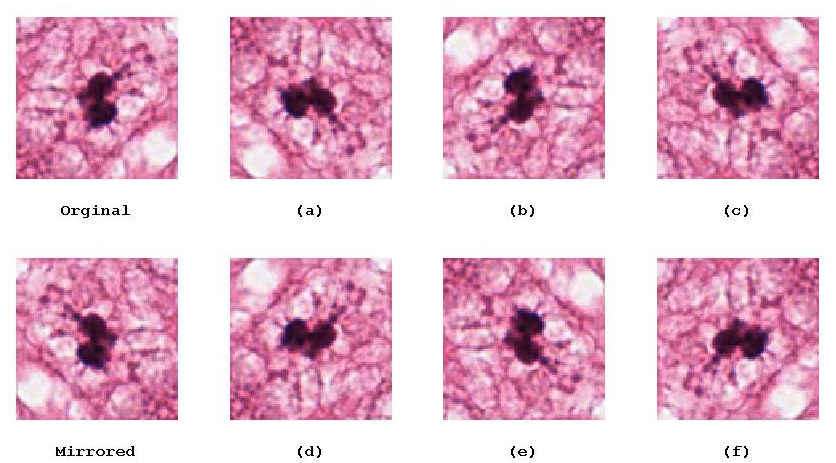
\includegraphics[width=0.96\textwidth]{./images/rotDataset_mod1.png}
  \caption[Extended Dataset]{Extended dataset\\(a),(b),(c): $\pi/2$ clockwise rotations, (d),(e),(f): mirror and $\pi/2$ clockwise rotations.}
  \label{ch4:fig1}
\end{figure}  

\vspace{0.5cm}




\section{Feature Extraction}
\label{ch4:FE}

Each image patch can be represented as a 100$\times$100$\times$3 matrix, where the $(i,j,:)$ triplet represents the RGB value of point with coordinates $(i,j)$ in the image.
Each value is in the range 0 to 255. Starting from these (raw) data we extracted some features by which we trained and tested our classifiers.

\vspace{0.5cm}

\subsection{Simple Features}
\label{ch4:sf}

The simplest features that can be computed involve the average and the standard deviation of the \Gls{RGB} values of the image patch. They can be computed on all the data or can be maintained separated
for each \Gls{RGB} component. In the first case, average and standard deviation each give one value every instance:

\begin{eqnarray}
 m & = & \frac{1}{100\cdot100\cdot3} \left( \sum_{i=1}^{100} \sum_{j=1}^{100} \sum_{k=1}^{3} i_{ijk} \right) \\
 \sigma & = & \sqrt{\frac{1}{100\cdot100\cdot3} \left( \sum_{i=1}^{100} \sum_{j=1}^{100} \sum_{k=1}^{3} (i_{ijk} - m )^2 \right)}
\end{eqnarray}

Otherwise, average and standard deviation produce a vector of three components:

\begin{eqnarray}
 \overline{M} & = & \left[ \begin{array}{c}
                            \frac{1}{100\cdot100} \left( \sum_{i=1}^{100} \sum_{j=1}^{100} i_{ij1} \right) \\
                            \frac{1}{100\cdot100} \left( \sum_{i=1}^{100} \sum_{j=1}^{100} i_{ij2} \right) \\
                            \frac{1}{100\cdot100} \left( \sum_{i=1}^{100} \sum_{j=1}^{100} i_{ij3} \right)
                           \end{array} \right] \\
 \overline{S} & = & \left[ \begin{array}{c}
                                 \sqrt{\frac{1}{100\cdot100} \left( \sum_{i=1}^{100} \sum_{j=1}^{100} (i_{ij1} - M(1) )^2 \right)} \\
                                 \sqrt{\frac{1}{100\cdot100} \left( \sum_{i=1}^{100} \sum_{j=1}^{100} (i_{ij2} - M(2) )^2 \right)} \\
                                 \sqrt{\frac{1}{100\cdot100} \left( \sum_{i=1}^{100} \sum_{j=1}^{100} (i_{ij3} - M(3) )^2 \right)}
                                \end{array}  \right]
\end{eqnarray}

Another simple set of features is represented by the \textit{median} of each \Gls{RGB} value. The median is defined as the numerical value separating the higher half of the data sample, from the lower half
and can be found by arranging all the data from lowest value to highest value and picking the middle one, or the mean of the two middle values, in case of even data.
Each of the features above are independent of the orientation of the image.
%	-	m: mean
%	-	s: standard deviation
%	-	M: mean per color
%	-	S: std per color
%	-	d: median per color



\vspace{0.5cm}

\subsection{Color Histograms and Intensities}
\label{ch4:chi}

A color histogram is a representation of the distribution of colors in an image, i.e. the number of pixels that have colors in each of a fixed list of color ranges \cite{colorHistogram01},
that span the image's color space. The color histogram can be built for any kind of color space, although the term is more often used for three-dimensional spaces like \Gls{RGB} or \Gls{HSV}.
A histogram of an image is produced first by discretization of the colors in the image into a number of bins, and counting the number of image pixels in each bin.
We built the \Gls{RGB} color histogram for each image patch, using 16 bins for each channel. The feature vector is so composed of 48 elements.\\
Also this feature is orientation independent.


\begin{figure}[!hbt]
  \centering
    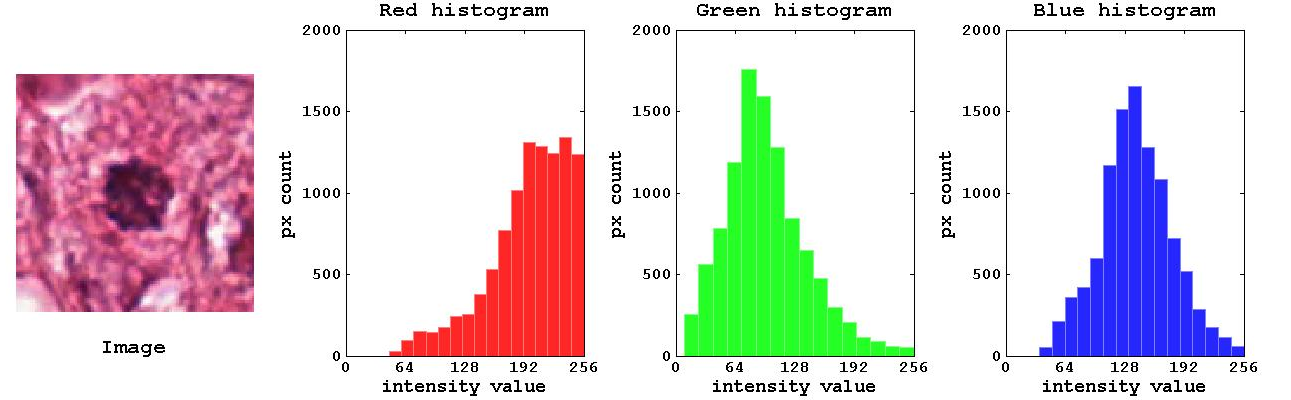
\includegraphics[width=0.98\textwidth]{./images/histIM_mod1.png}
  \caption[Color Histograms]{Color Histograms of sample image}
  \label{ch4:fig2}
\end{figure}  

It is generally possible to transform a color image into a gray-scale one. One typical transformation algorithm, applied pixel by pixel, is the following:

\begin{equation}
 \label{ch4:eqGS}
 pix_{gray} = 0.2989 \cdot pix_{red} + 0.5870 \cdot pix_{green} + 0.1140 \cdot pix_{blue}
\end{equation}

On the resulting monochromatic image, it is possible to compute an \textit{intensity histogram}.\\
We preferred to compute a slightly different feature: the average intensity in the 25 central regions of the image.
We first computed the gray-scale image according to Equation \ref{ch4:eqGS}, then we selected the central part of the image and divided it in a grid of $5\times5$ elements.
We finally computed the mean intensity for each element. Figure \ref{ch4:fig3} illustrates the procedure.

\begin{figure}[!hbt]
  \centering
    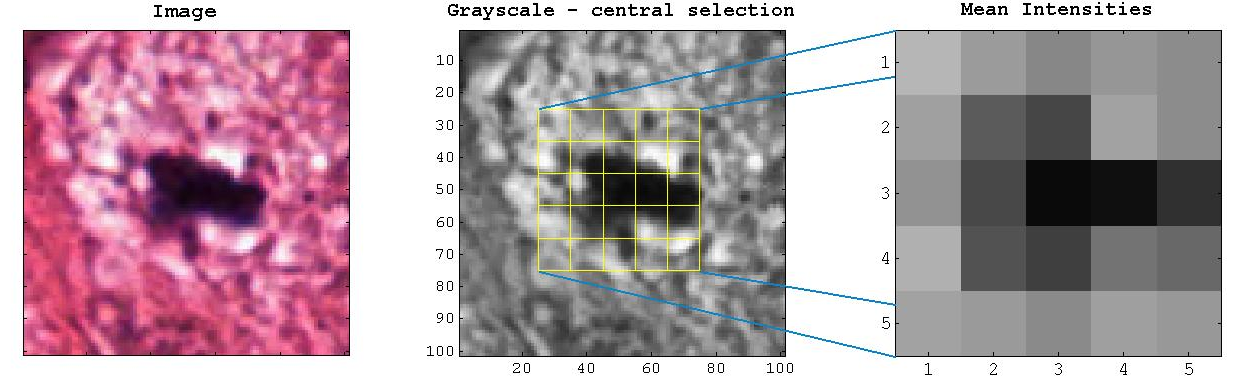
\includegraphics[width=0.99\textwidth]{./images/GSintens1_mod1.png}
  \caption[Example of mean gray-scale intensities feature]{Mean gray-scale intensity of central part of image patch}
  \label{ch4:fig3}
\end{figure}

The resulting feature vector is composed of 25 values, corresponding to the intensities, ordered columnwise. This type of feature is orientation dependent.

%	-	H: color histograms (16 bins)
%	-	i: mean intensity in 25 central regions of the image


\vspace{0.5cm}

\subsection{Texture Features}
\label{ch4:tf}

Texture features are widely used in different \Gls{CV} tasks, as pointed out in Section \ref{ch2:texture}. We focused on the features based on Local Binary Patterns (\Gls{LBP}),
described in \cite{LBP01} and \cite{LBP02}. The general idea of \Gls{LBP} is described on page \pageref{ch2:lbp}.
The \Gls{LBP} features considered here are labeled LBP$_{P,R}$ where \textit{P} is the number of neighbors considered and \textit{R} is the distance from the pixel.
The two main characteristics of the \Glspl{LBP} considered are:

\begin{itemize}
 \item \textit{uniformity}: which is a fundamental property of local image texture. It refers to the uniform appearance of the local
binary pattern: that is, there is a limited number of transitions or discontinuities in the circular presentation of the pattern.
The most frequent uniform binary patterns correspond to primitive \textquotedblleft microfeatures\textquotedblright, such
as edges, corners, and spots; hence, they can be regarded as feature detectors that are triggered by the best matching
pattern.
\item \textit{rotation invariance}: which takes into account if a spatial pattern is affected by rotation or not.
\end{itemize}

Three different types of features can be built, on the basis of the relations described Equation \ref{ch2:eq_lbp1}:

\begin{enumerate}
 \item $\text{LBP}_{P,R}^{u2}$: uniform feature,
 \item $\text{LBP}_{P,R}^{ri}$: rotation invariant feature,
 \item $\text{LBP}_{P,R}^{riu2}$: uniform and rotation invariant feature,
\end{enumerate}

\noindent In particular we used:

\begin{equation}
 \text{LBP}_{8,R}^{\text{type}} \quad \textrm{where} \begin{cases}
    \text{type}  & \in \{ri, u2, riu2\}\\
    R  & \in \{1,2,3\}
  \end{cases}
\end{equation}

\noindent while building the feature vector, we used the \textit{type} parameter in a mutually exclusive way, i.e. we did not concatenate \Glspl{LBP} of different types. On the other hand, we
built feature vectors with various combitations of radii.\\
The following equations show the three different mutually exclusive texture feature sets that we considered.

\begin{eqnarray}
\label{ch4:tftypes}
 \overline{L} & = & \left[ \text{LBP}_{8,1}^{riu2}, \text{LBP}_{8,2}^{riu2}, \text{LBP}_{8,3}^{riu2} \right] \\
 \overline{U} & = & \left[ \text{LBP}_{8,1}^{u2}, \text{LBP}_{8,2}^{u2}, \text{LBP}_{8,3}^{u2} \right] \\
 \overline{R} & = & \left[ \text{LBP}_{8,1}^{ri}, \text{LBP}_{8,2}^{ri}, \text{LBP}_{8,3}^{ri} \right]
\end{eqnarray}

Finally, we considered the \Gls{VAR} operator, as described in Equation \ref{ch2:eq_lbp2}. As, from early tests, a single \Gls{VAR} value for the entire image patch proved to be non-significant, we
decided to follow an approach similar to the one described for the intensity histogram (see Figure \ref{ch4:fig3}) and evaluated the mean value of a grid of samples in the central
region of the image. Figure \ref{ch4:fig4} shows a sample of VAR(8,1) computation. Please note that the gray-scale mapping of the VAR(8,1) figure has been adjusted to be visible with full gray-scale range.

\begin{figure}[!hbt]
  \centering
    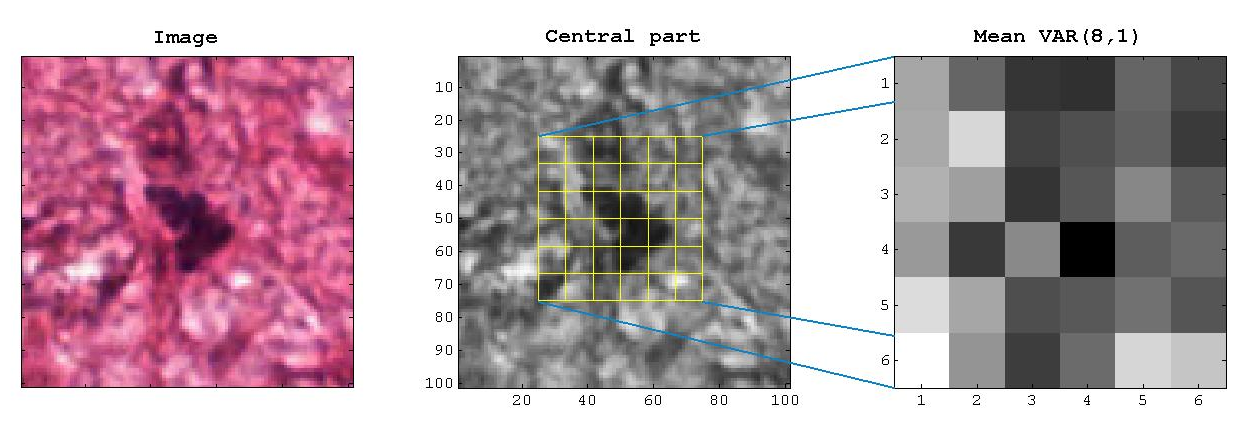
\includegraphics[width=0.94\textwidth]{./images/GS_VAR_mod1.png}
  \caption[Example of VAR(8,1) feature]{Example of VAR(8,1) feature}
  \label{ch4:fig4}
\end{figure}

The resulting feature vector is composed of 36 values, corresponding to the average VAR(8,1) in each element of the grid, ordered columnwise. This type of feature is orientation dependent.
\\
The Matlab code implemented to build the feature vectors can be found at \url{https://github.com/Ccaccia73/mitosis-experiments}, into the sub-directory \texttt{common},
function \texttt{extractFeatures.m}.


% \clearpage

%	-	l: lbp riu2 radius 1, 8 neighbors
%	-	r: lbp ri radius 1, 8 neighbors
%	-	u: lbp u2 radius 1, 8 neighbors
%	-	v: mean pixel variance
%	-	L: lbp riu2 radius 1-2-3, 8 neighbors concatenated
%	-	V: pixel variance, 36 elements
%	-	R: lbp ri radii 1-2-3, 8 neighbors
%	-	U: lbp u2 radii 1-2-3, 8 neighbors



\vspace{0.5cm}

%\clearpage

\section{Classifiers}
\label{ch4:classifiers}

Once defined the set of feature to be considered, it is possible to build a matrix whose lines represent an \textit{instance} (i.e. an image patch) and whose columns represent a \textit{feature}
(or a component of it): Equation \ref{ch4:fmat} represents such matrix.
\begin{equation}
\label{ch4:fmat}
 M_{feats} = \\ \bordermatrix{~ & \tikzmark{harrowleft} 1 & \cdots & ~  & \cdots & ~ & \cdots & ~ & n_{fc}\tikzmark{harrowright}  \cr
			      \tikzmark{varrowtop} 1 & c_{111} & c_{112} & \cdots & c_{1k1} & \cdots & c_{1kn_k} & \cdots & c_{1n_f1} \cr
			                      \vdots &    ~    &   ~     &   ~    &    ~    &   ~    &     ~     &    ~   &     ~     \cr
			                       ~     & \vdots  & \vdots  & \ddots & \vdots  & \ddots & \vdots    & \ddots &  \vdots   \cr
			                      \vdots &    ~    &   ~     &   ~    &   ~     &   ~    &    ~      &    ~   &    ~      \cr
			      \tikzmark{varrowbottom} n_i & \tikzmark{f1} c_{n_i11} & c_{n_i12} \tikzmark{f2} & \cdots & \tikzmark{f3} c_{n_ij1} & \cdots & c_{n_ijn_j} \tikzmark{f4} & \cdots & \tikzmark{f5} c_{n_in_f1} \tikzmark{f6} \cr
			     }
\end{equation}
\tikz[overlay,remember picture] {
  \draw[->] ([yshift=3ex]harrowleft) -- ([yshift=3ex]harrowright)
            node[midway,above] {\tiny \textit{features}};
  \draw[->] ([yshift=1.5ex,xshift=-0.8ex]varrowtop) -- ([xshift=-0.8ex]varrowbottom)
            node[pos=0.0,anchor=north,xshift=-0.65cm,yshift=-2.3cm] {\tiny \textit{instances}};
  \draw [thick, decoration={ brace, amplitude=8pt, mirror, raise=0.12cm}, decorate] (f1) -- (f2) 
	    node [pos=0.5,anchor=north,yshift=-0.36cm] {\tiny \textit{feat$_1$}};
  \draw [thick, decoration={ brace, amplitude=8pt, mirror, raise=0.12cm}, decorate] (f3) -- (f4) 
	    node [pos=0.5,anchor=north,yshift=-0.36cm] {\tiny \textit{feat$_j$}};
  \draw [thick, decoration={ brace, amplitude=5pt, mirror, raise=0.12cm}, decorate] (f5) -- (f6) 
	    node [pos=0.5,anchor=north,yshift=-0.36cm] {\tiny \textit{feat$_{nf}$}};
}

\noindent Where $n_f$ is the total number of features and $n_i$ is the total number of instances. Each feature can be made of more than one component (e.g. $feat_1$ and $feat_j$ in the example).
For this reason, the total number of columns in the matrix $(n_{fc})$ is given by the sum of all the feature components. So, 
each element of the matrix $c_{ijk}$ is the $k^{th}$ component of the $j^{th}$ feature in the $i^{th}$ instance. The matrix representing the eavluation set is built in the same way.\\
A vector represents the class which every instance belongs to. Equation \ref{ch4:cvect} describes such vector:
\begin{equation}
\label{ch4:cvect}
 V_{class} = \\ \bordermatrix{~ &  ~  \cr
			      \tikzmark{varrowtop} 1 &  \tikzmark{f5} e_{1}  \tikzmark{f6} \cr
			                      \vdots & \vdots \cr
			                       ~     & e_i   \cr
			                      \vdots & \vdots \cr
			      \tikzmark{varrowbottom} n_i & e_{n_i} \cr
			     }
\end{equation}
\tikz[overlay,remember picture] {
  \draw[->] ([yshift=1.5ex,xshift=-0.8ex]varrowtop) -- ([xshift=-0.8ex]varrowbottom)
            node[pos=0.0,anchor=north,xshift=-0.65cm,yshift=-2.3cm] {\tiny \textit{instances}};
  \draw [thick, decoration={ brace, amplitude=3pt, raise=0.25cm}, decorate] (f5) -- (f6) 
	    node [pos=0.5,anchor=north,yshift=0.76cm] {\tiny \textit{class}};
}

where $e_i$ belongs to one of the two classes. In some implementations of binary classifiers it is required that $e_i \ \in \{-1,1\} \ \forall i = 1,\cdots,n_i$,
otherwise $e_i \ \in \{0,1\} \ \forall i = 1,\cdots,n_i$. The vector 
representing the \Gls{GT} of the evaluation set is built in the same way.\\
Having a matrix representing the training feature set, a matrix representing the evaluation (i.e. testing) feature set and two vectors including the \Gls{GT}
classification of each image patch, it is possible to run a classifier that tries to get insights form the feature set in order to classify the evaluation set.\\


In our work we focused on two types of classifiers:

\begin{itemize}
 \item \textit{Support Vector Machines}, which are widely used in computer vision classification problems, in particular
in biomedical imaging (\cite{mitosisDetectionLearningBased, SVM02, SVM03, SVMClassHistogram}, see also Section \ref{ch3:review}),
 \item \textit{Random Forests}, which is a relatively new ensemble approach that can also be thought of as a form of nearest neighbor predictor (\cite{randForests03,randForests02,randForests04}).
\end{itemize}

We also mention \Gls{CNN}, as it played a relevant role in the definition of our dataset (see Section \ref{ch4:ic}).


\vspace{0.5cm}

\subsection{Support Vector Machines}
\label{ch4:svm}

We used the Matlab implementation of the \textit{libSVM} described in \cite{SVM01}. \Glspl{SVM} are a popular classification technique.
The goal of \Gls{SVM} is to produce a model (based on the training data) which predicts the target values of the test data
given only the test data attributes. Given a training set of instance-label pairs $(\mathbf{x_i}, y_i)$, $i = 1,\cdots,l$, where $\mathbf{x_i} \in \mathbb{R}^n$ and $y \in \{-1,1\}^l$.\\
The \Gls{SVM} requires the solution of the following optimization problem:

\begin{equation}
     \begin{aligned}
      \smash{\min_{\textbf{w},b,\xi}} \quad & \frac{1}{2}\textbf{w}^T\textbf{w}+C \sum_{i=1}^{l}\xi_i   \\
      \text{Subject to:} &\\
       & y_i \left(\textbf{w}^T \phi( \mathbf{x_i} ) +b\right) \geq 1-\xi_i \\
       & \xi_i \geq 0 
     \end{aligned}
     \phantom{\hspace{3cm}} %%<---adjust the value as you want
\end{equation}

The training vectors $\mathbf{x_i}$ are mapped into a higher dimensional space (maybe infinite), by the function $\phi$.
\Gls{SVM} finds a linear separating hyperplane with the maximal margin in this higher dimensional space.
$C > 0$ is the penalty parameter of the error term.
The function

\begin{equation}
 K(\mathbf{x_i}, \mathbf{x_j}) = \phi(\mathbf{x_i})^T\phi(\mathbf{x_j})
\end{equation}

is called the \textit{kernel function}. Many kernel functions have been defined, the most common are:

\begin{itemize}
 \item \textit{linear}: $K(\mathbf{x_i}, \mathbf{x_j}) = \mathbf{x_i}^T\mathbf{x_j}$,
 \item \textit{polynomial}: $K(\mathbf{x_i}, \mathbf{x_j}) = \left(\gamma \mathbf{x_i}^T\mathbf{x_j} + r \right)^d, \gamma > 0$,
 \item \textit{\Gls{RBF}}: $K(\mathbf{x_i}, \mathbf{x_j}) = \exp{\left(-\gamma \lVert \mathbf{x_i} - \mathbf{x_j} \rVert^2 \right)}, \gamma > 0$,
 \item \textit{sigmoid}: $K(\mathbf{x_i}, \mathbf{x_j}) = \tanh \left( \mathbf{x_i}^T\mathbf{x_j} + r \right)$.
\end{itemize}

Where $\gamma$, \textit{d} and \textit{r} are kernel parameters \cite{ML01}.\\
In our work we focused on \Glspl{RBF} and sigmoid kernels, which are used in most cases.
In \Glspl{SVM} the \textit{support vectors} are the training instances that concur to define the separating hyperplane in the kernel space. The 
image of Figure \ref{ch4:fig5} gives a linear representation of a \Gls{SVM}.

\begin{figure}[!hbt]
  \centering
    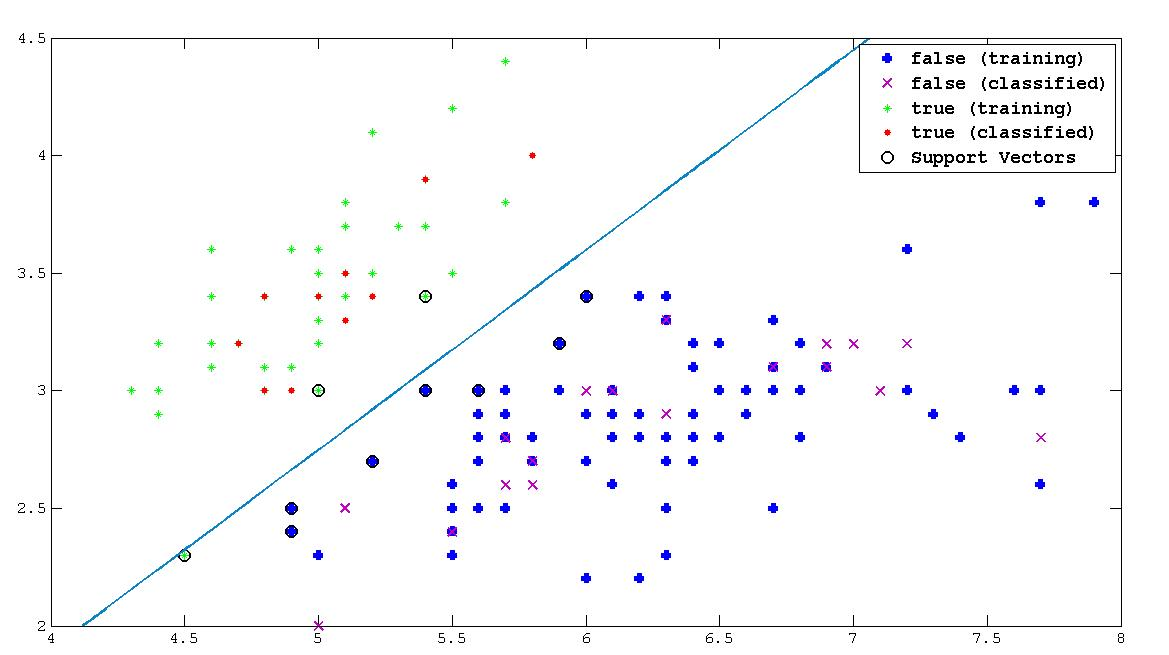
\includegraphics[width=0.98\textwidth]{./images/SVM_example_mod1.png}
  \caption{Representation of a SVM classification}
  \label{ch4:fig5}
\end{figure}


\vspace{0.5cm}

\subsection{Random Forests}

\Glspl{DT} are attractive classifiers due to their high execution speed and simplicity. However, trees often suffer from performance loss, in terms
of generalization accuracy on unseen data when the complexity of the problem grows \cite{randForests01}.\\
Random Forests are a combination of tree predictors such that each tree depends on the values of a
random vector sampled independently and with the same distribution for all trees in the forest \cite{randForests03}.
So, \Gls{RF} can be viewed as an ensemble approach that can also be thought of as a form of nearest neighbor predictor.
Ensembles are a divide-and-conquer approach used to improve performance. The main principle behind ensemble methods is that a group of \textquotedblleft weak learners\textquotedblright
can be combined together to form a \textquotedblleft strong learner\textquotedblright. Each classifier, individually, is a weak learner, while all the classifiers taken together are a strong learner.
An example of \Gls{DT} is shown in Figure \ref{ch4:fig6}.

\begin{figure}[!hbt]
  \centering
    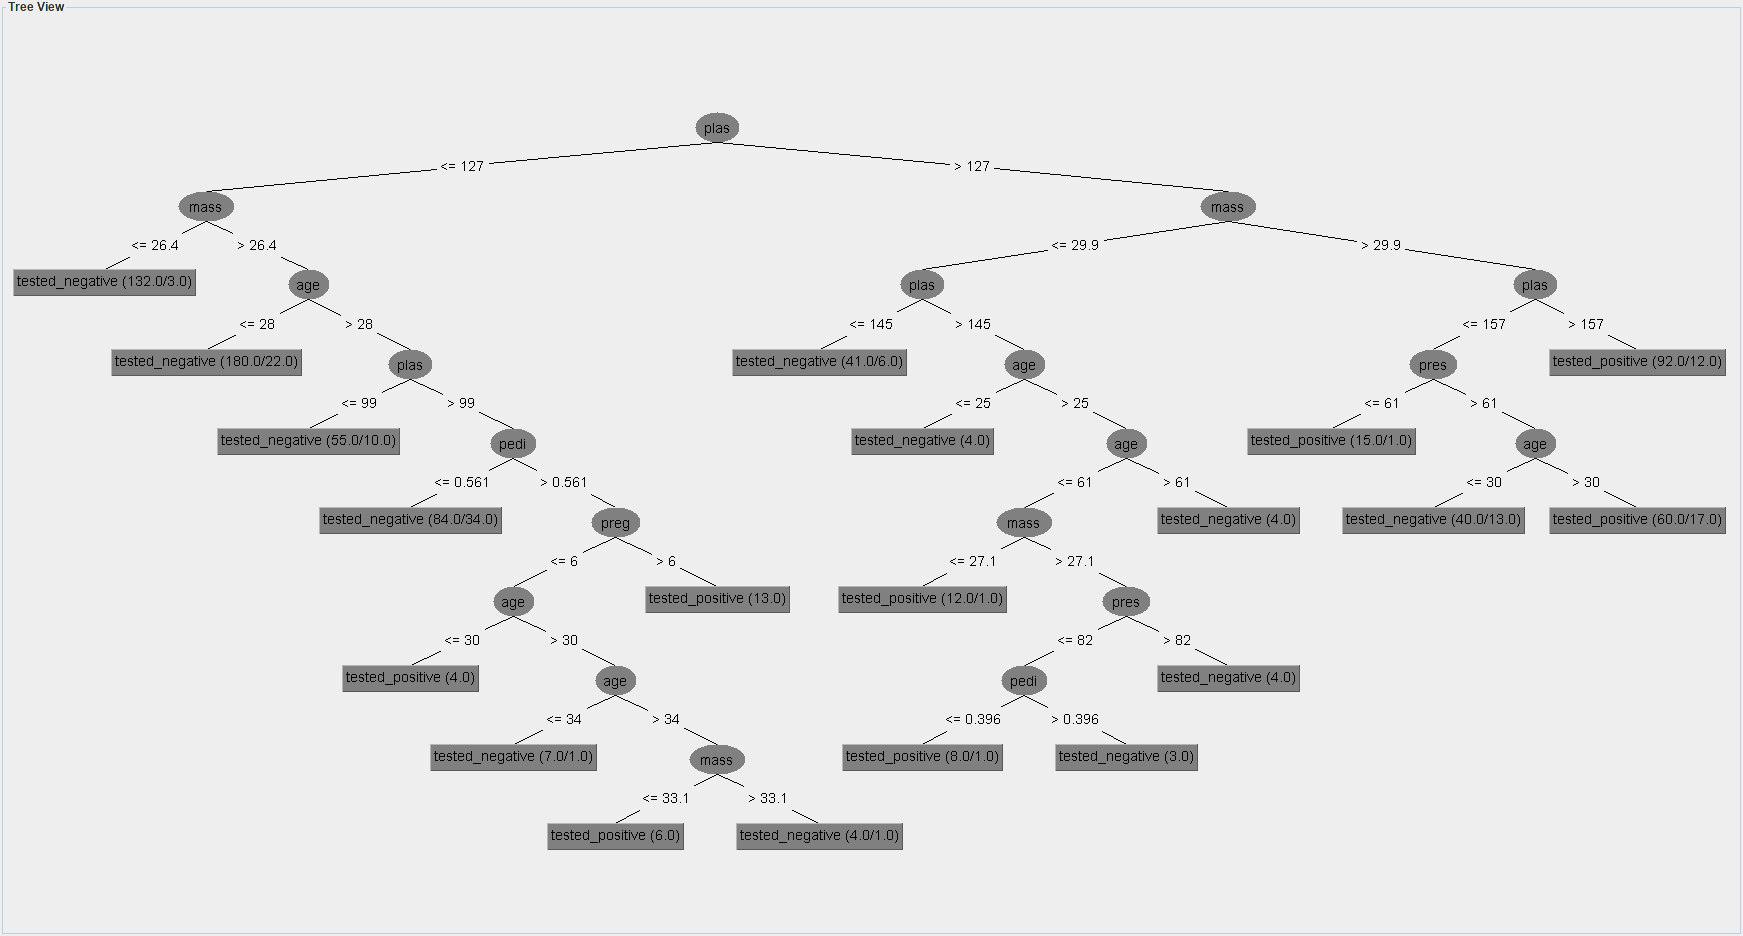
\includegraphics[width=0.98\textwidth]{./images/DT_example.png}
  \caption{Example of a Decision Tree}
  \label{ch4:fig6}
\end{figure}

A \Gls{RF} is composed by a number of trees \textbf{T}. For some number \textit{m}, \textit{m} features are randomly selected from the feature vector.
The subset of variables is used to train a \Gls{DT}.\\
According to Breiman implementation of \Glspl{RF}, \textit{m} should be that  $\ll$ than the number of features.\\
We adopted the convention (as described in \cite{randForests03}) that $m \leq \log_2 F +1$ and used an ensemble of 500 trees.\\
While running a \Gls{RF}, when a new input is entered into the system (a test sample), it is run down all of the trees, each of which classifies
it in a \textit{hard} way (see Section \ref{ch3:class}): in a sense, each tree gives a vote for the current sample. 
The result is the average  of all of the terminal nodes that are reached, giving a final \textit{soft} classification.
\Glspl{RF} are generally quite fast, robust classifiers, and are also used in image classification \cite{randForests04}.
\\
The Matlab code implemented to classify data can be found in function \texttt{classifyData.m} in the same repository.

\vspace{0.5cm}


\section{Classification Process}

Once a classifier is trained on the training set, it can be used to classify unseen data (i.e., the evaluation or testing set). The classifier
function is applied to each instance of the \textit{evaluation} feature set, which is built as the matrix described in Equation \ref{ch4:fmat}.\\
The output of the classifier is a vector like the one described in Equation \ref{ch4:cvect}, unless that, generally, the classification
process gives a \textit{soft} classification (see Section \ref{ch3:class}), which means that  $-1 \leq e_i \leq 1 \ \forall i = 1,\cdots,n_i$, or
$0 \leq e_i \leq 1$, depending on the definition of the classes.\\
The performance parameters are computed as a function of a \textit{classification threshold}, as described in Section \ref{ch3:roc}.



% In most computer vision applications it is not sufficient to extract only one type of feature to obtain the relevant information from the image data.
% Instead two or more different features are extracted, resulting in two or more feature descriptors at each image point.
% A common practice is to organize the information provided by all these descriptors as the elements of one single vector,
% commonly referred to as a feature vector. The set of all possible feature vectors constitutes a feature space.
% A common example of feature vectors appears when each image point is to be classified as belonging to a specific class.
% Assuming that each image point has a corresponding feature vector based on a suitable set of features,
% meaning that each class is well separated in the corresponding feature space, the classification of each image point can be done using standard classification method.

 



\chapter{Design of a User Study}
\label{chapter5}
\thispagestyle{empty}

\begin{quotation}
{\footnotesize
\noindent \emph{``Terence: Ma scusa di che ti preoccupi, i piedipiatti hanno altro a cui pensare, in questo momento stanno cercando due cadaveri scomparsi \\
Bud: Se non spegni quella sirena uno di quei due cadaveri scomparsi lo trovano di sicuro!''}
\begin{flushright}
Nati con la camicia
\end{flushright}
}
\end{quotation}
\vspace{0.5cm}

\noindent Si mostra il progetto dell'architettura del sistema con i vari moduli.

\chapter{Experimental Results}
\label{chapter6}
\thispagestyle{empty}

\begin{quotation}
{\footnotesize
\noindent\emph{``Quote 6''}
\begin{flushright}
Author 6
\end{flushright}
}
\end{quotation}

\vspace{0.5cm}

%\noindent Si mostra il progetto dal punto di vista sperimentale, le cose materialmente realizzate. In questa sezione si mostrano le attivit\`a sperimentali svolte, si illustra il funzionamento del sistema (a grandi linee) e si spiegano i risultati ottenuti con la loro valutazione critica. Bisogna introdurre dati sulla complessit\`a degli algoritmi e valutare l'efficienza del sistema.

\section{Accuracy of the Detection Algorithm}

\vspace{0.5cm}

\section{Accuracy of Humans}

\vspace{0.5cm}

\section{Accuracy of Algorithms}

(rif. paper)

\subsection{Performances of Algorithms on MITOS Dataset}
\label{ch6:icpr_perf}

We report here the performances of the best-scoring algorithms that participated to the ICPR2012 Contest, as shown on the contest website (Figure \ref{ch6:fig3}).
The principal metric adopted to compare algorithms is the $F_1$-Score (Figure \ref{ch6:fig3:a}) , but also precision and recall are shown \ref{ch6:fig3:b}. 

\begin{figure}[!htb]
  \centering
    \subfigure[F-Score]{
      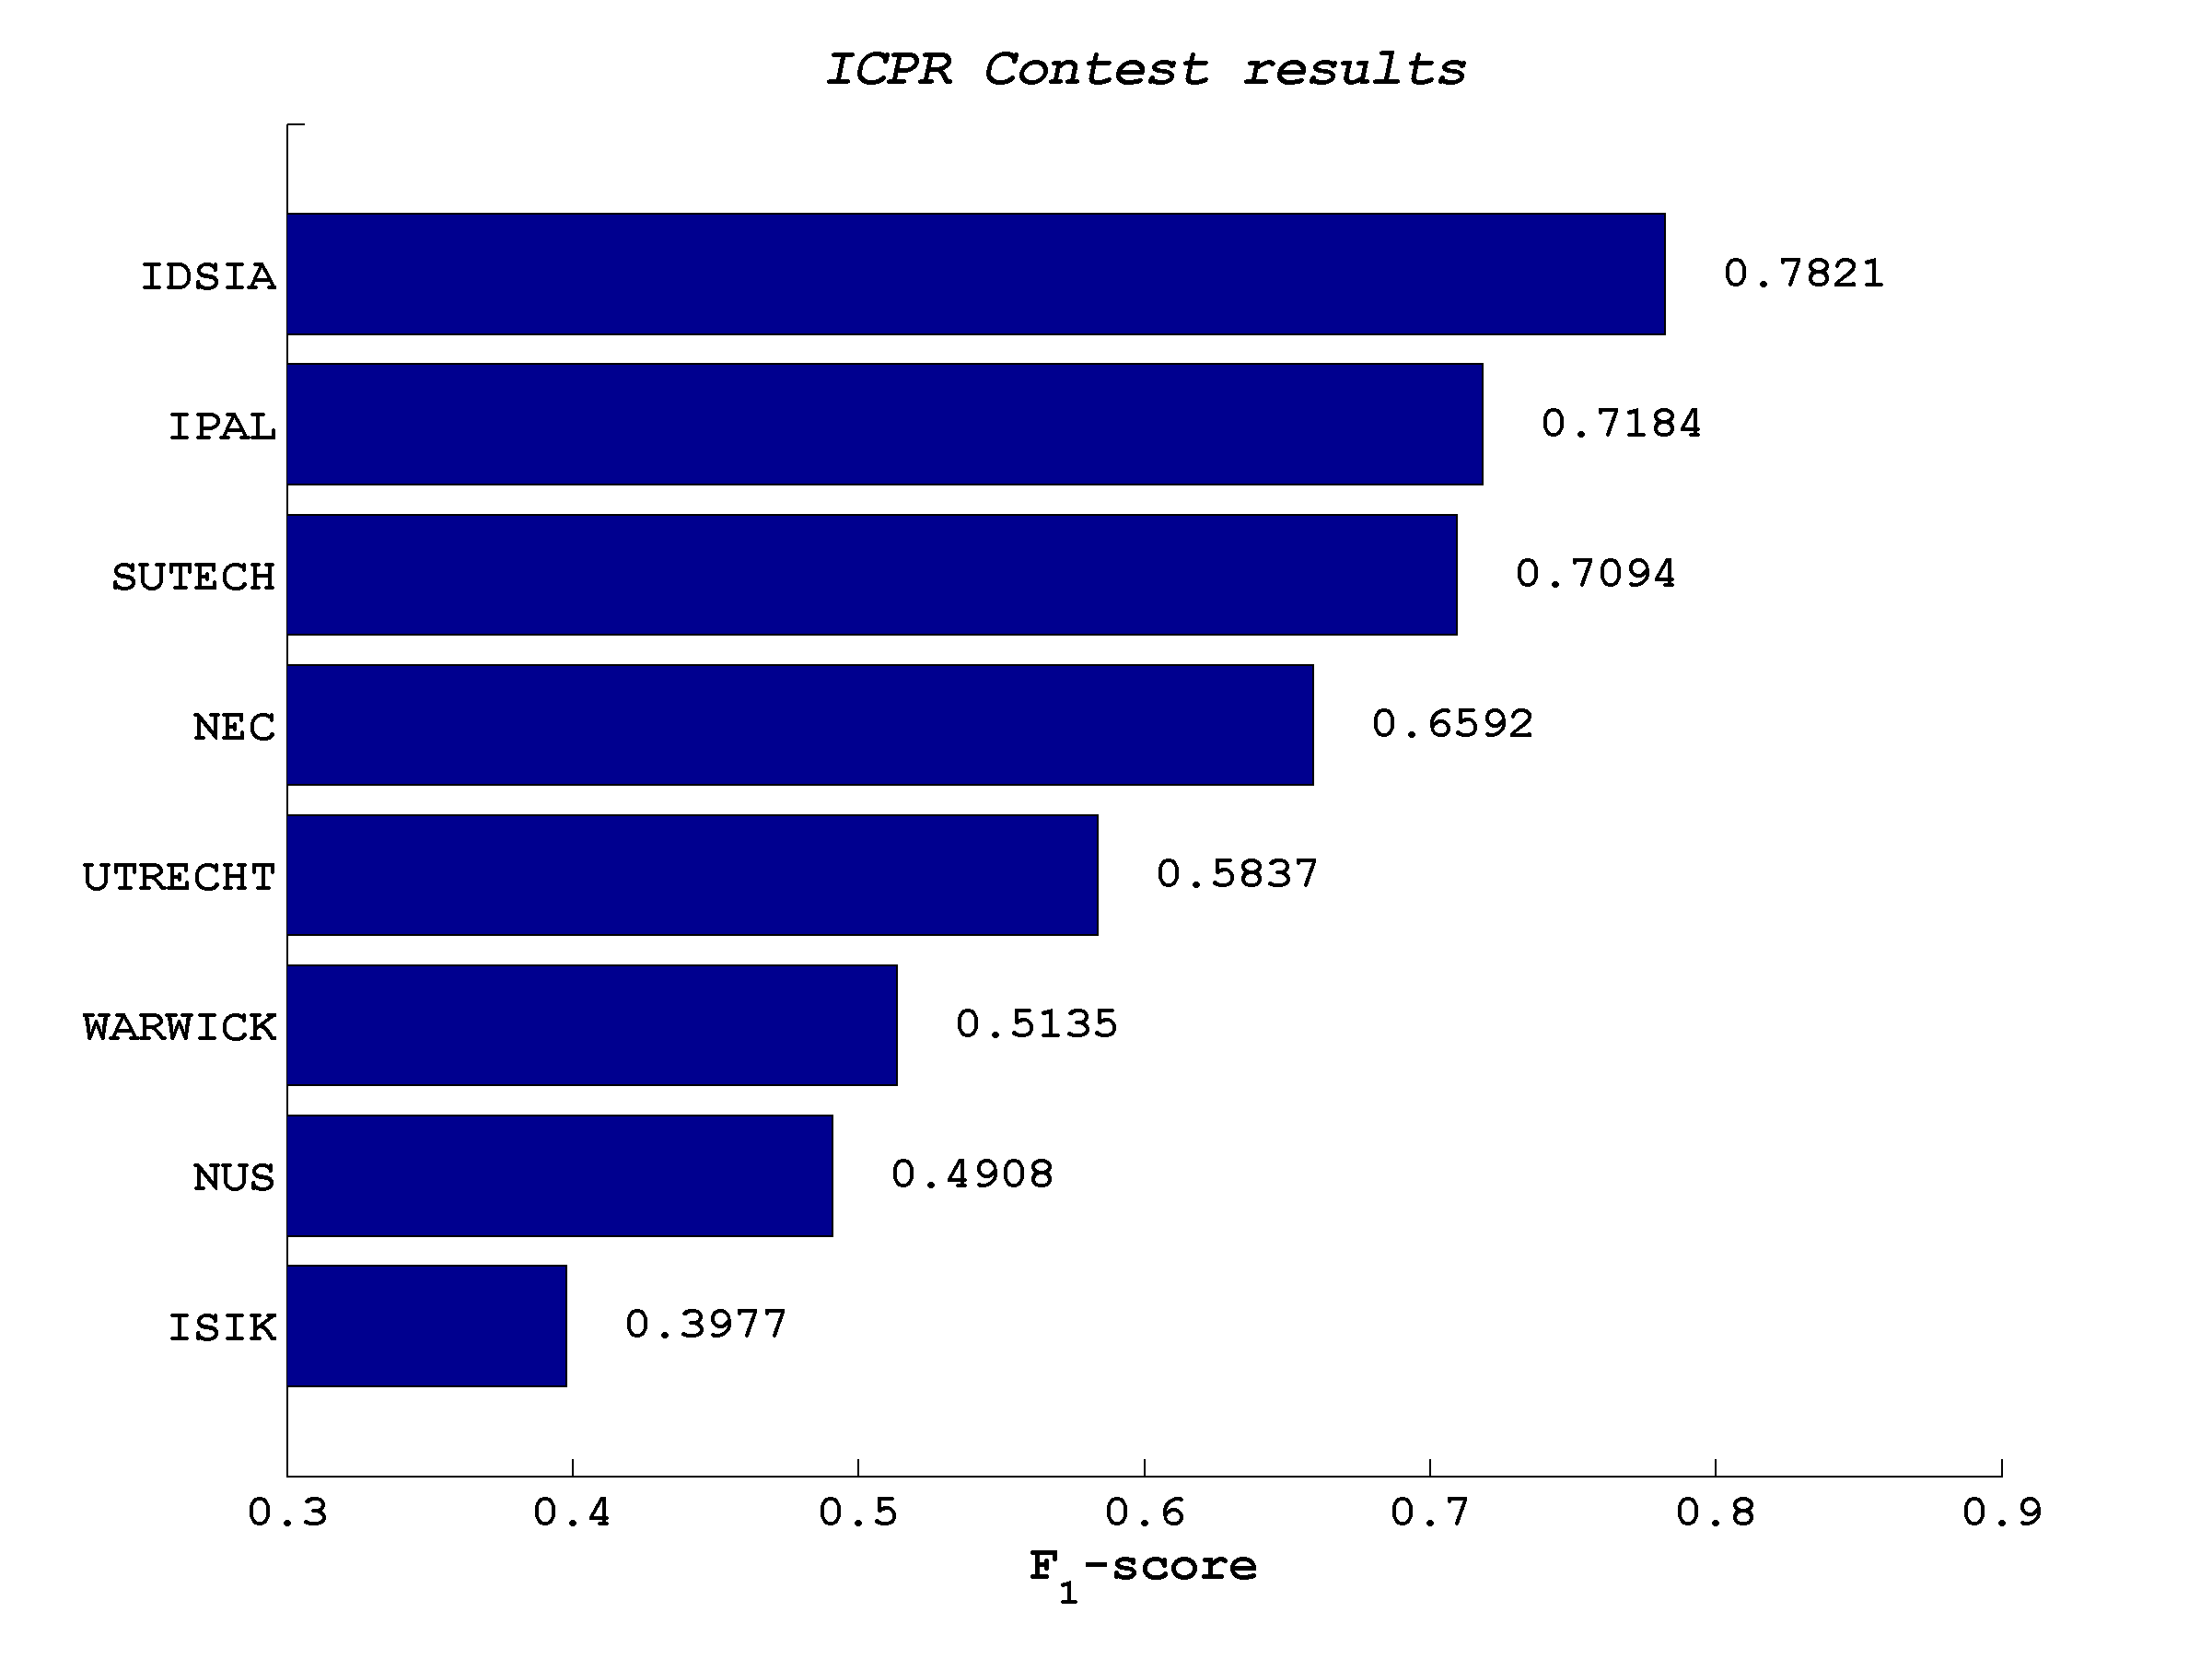
\includegraphics[width=0.82\textwidth]{./images/ICPRperf1.png}
      \label{ch6:fig3:a}
    }\\
    %\hspace{1mm}
    \subfigure[metrics]{
      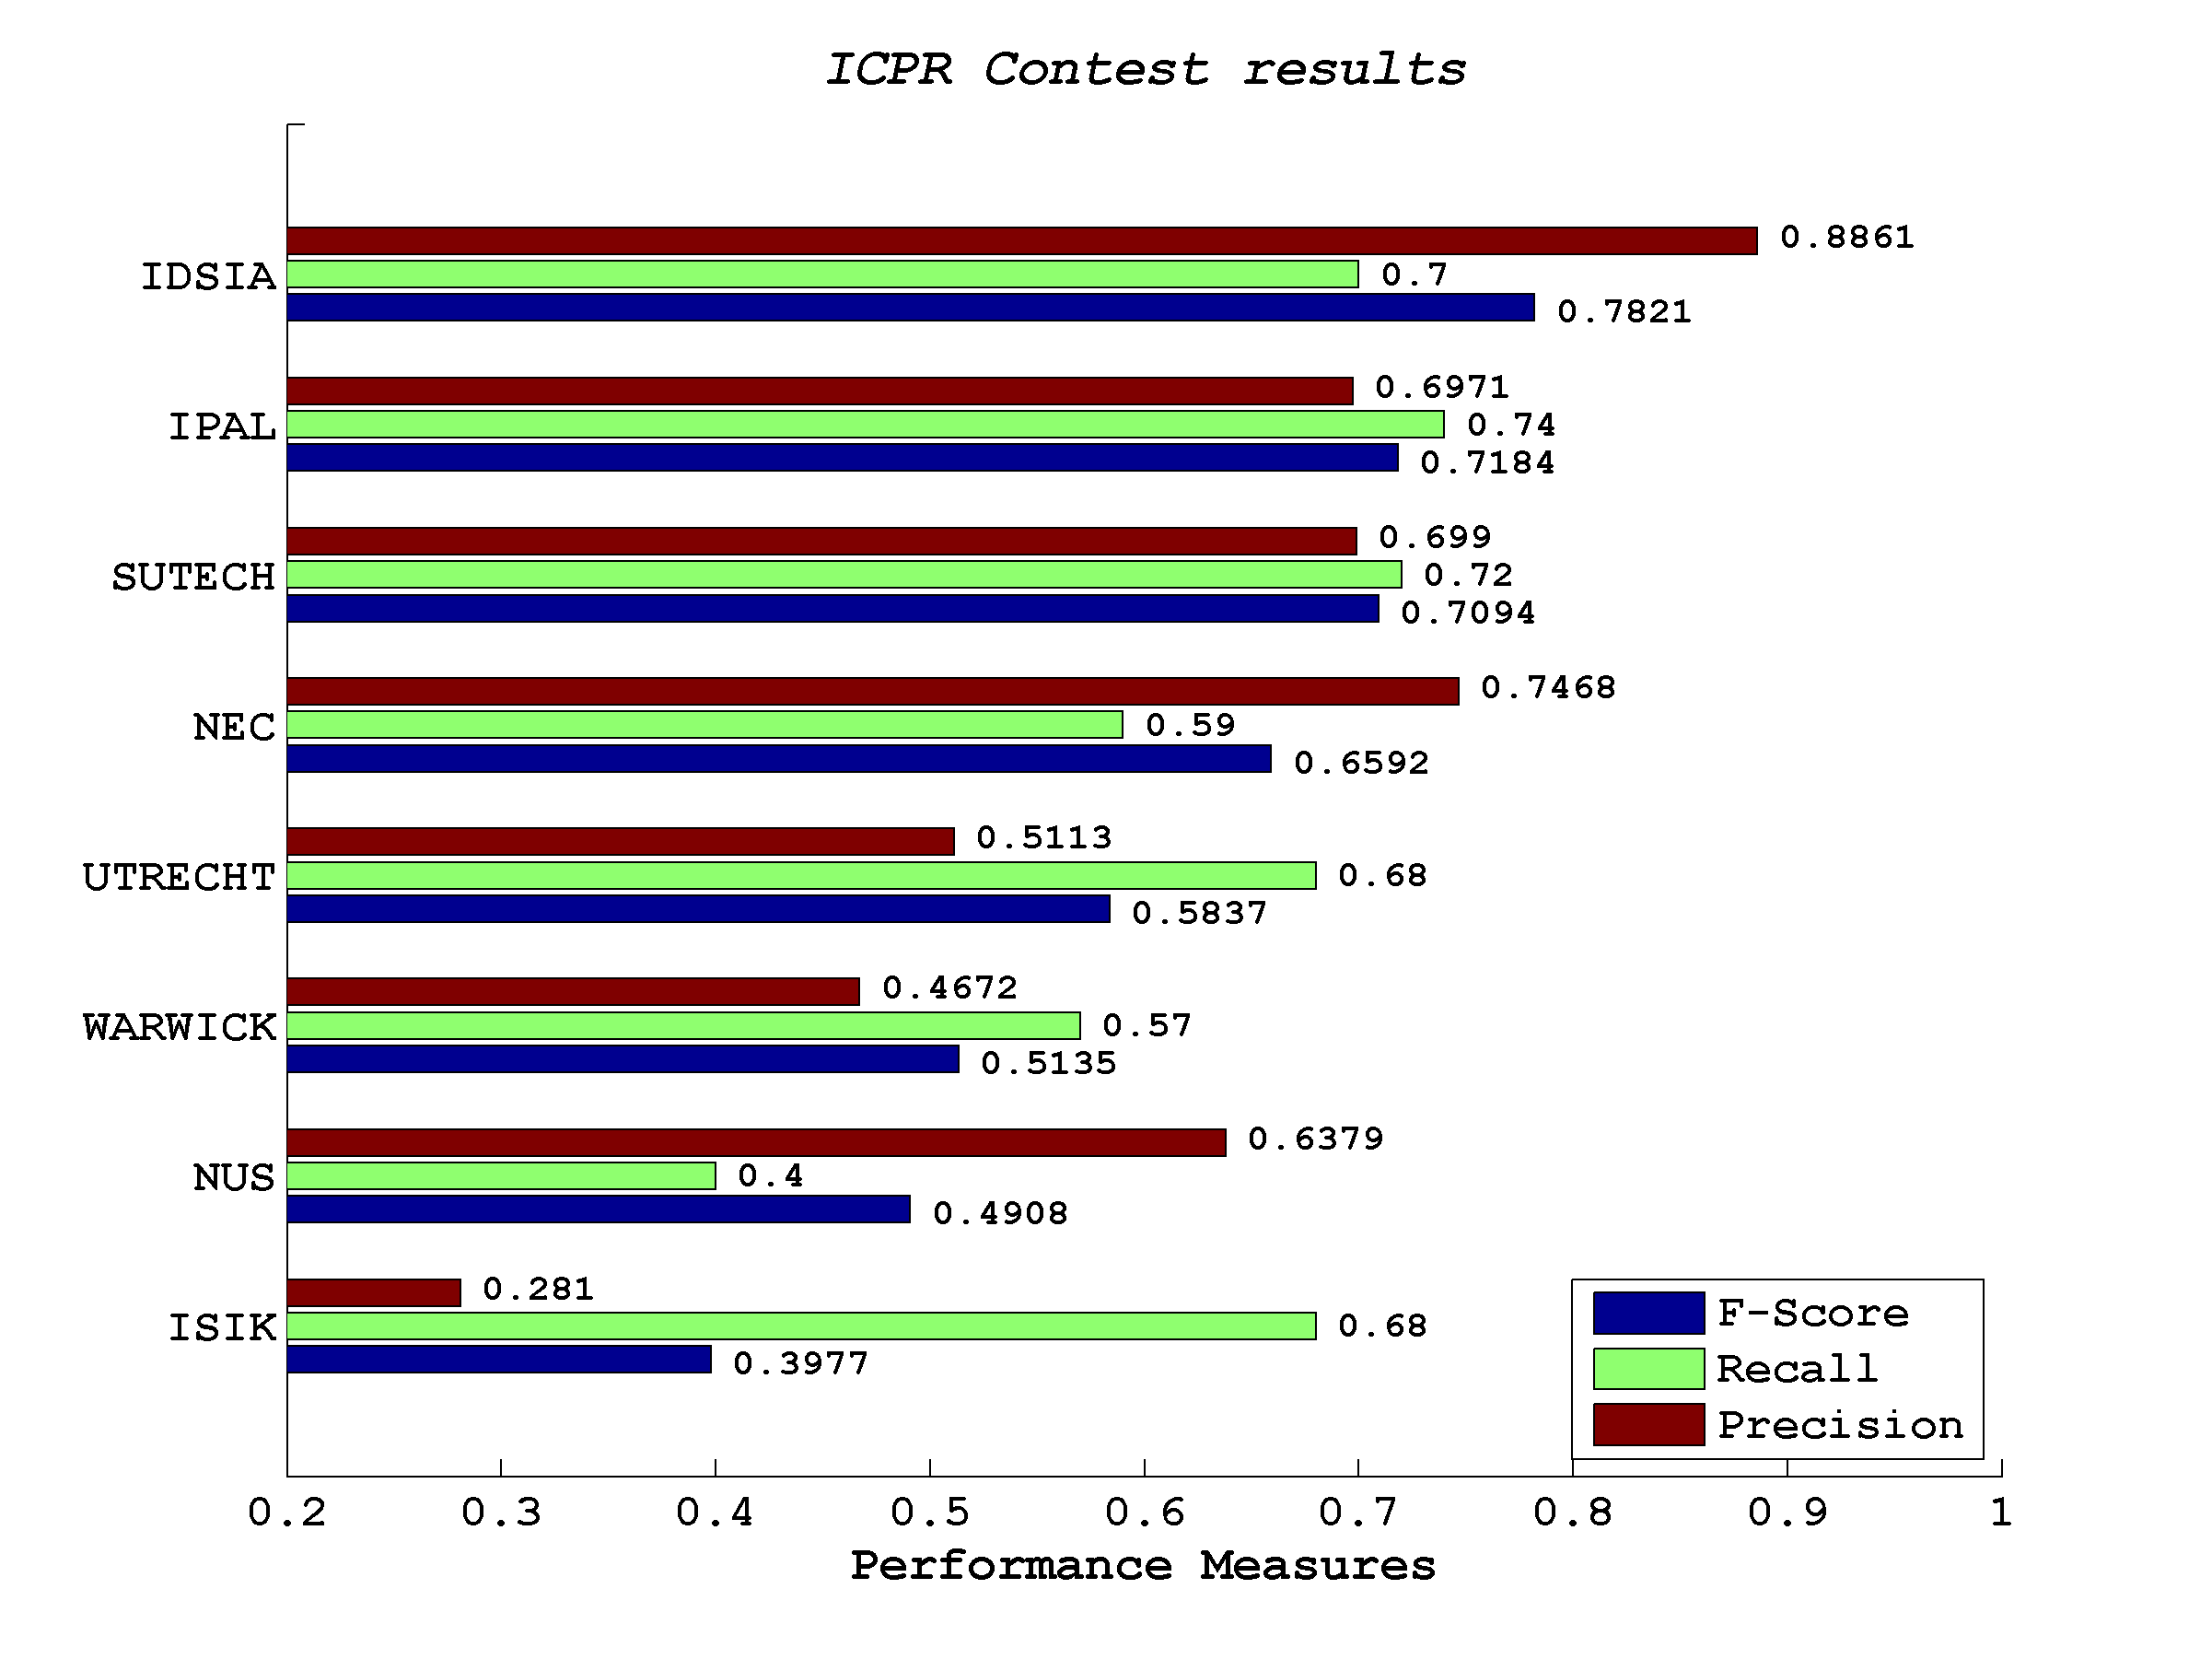
\includegraphics[width=0.82\textwidth]{./images/ICPRperf2.png}
      \label{ch6:fig3:b}
    }
    \caption{Performances of best algorithms in ICPR 2012 contest}
    \label{ch6:fig3}
\end{figure}
\chapter{Conclusions}
\label{chapter7}
\thispagestyle{empty}


\begin{quotation}
{\footnotesize
\noindent{\emph{``\greek{di`o o>ud'epote noe~i >'aveu fant'asmatoc <h yuq'h}''}\\
(The soul never thinks without a picture)}
\begin{flushright}
\greek{>Aristot'elhc} (Aristotle, On the Soul 4.7.431a16)
\end{flushright}
}
\end{quotation}

\vspace{0.5cm}


\section{Context and Results}

Breast cancer is one of the most deadly cancers for women. According to the increasing incidence rate of breast
cancer reported in many countries, early cancer detection and treatment play a major role
in increasing the chances of recovery from the disease. Nottingham Grading
System \Gls{NGS} is the standard grading procedures used in breast cancer assessment;
it focuses on three criteria: Mitotic Count , Nuclear Pleomorphism , and
Tubule Formation. Each criterion can be assigned with 3 scores, and the final
equivalent NGS grade is the summation of all three criteria.\\
Breast tissue samples of patients are taken for grading by means of biopsy. The \Gls{NGS} grade
of tissue samples are based on the deviation of the cell structures from normal
tissues.\\
Pathologists need to assess lots of tissue samples under the microscope every day.
Low agreement for medical cases is typical between pathologists
because they exam breast tissue samples based on their experience and opinion.
Hence, the evaluation of breast cancer grading is a subjective, manual, and
time-consuming process.\\
Digital high resolution histo-pathological images are commonly used for extracting useful structural information from samples
With the rapid growth in computer technologies, many computer science researches have
focused on computer aided diagnosis (\Gls{CAD}) systems to develop a standard and
quantitative measurement for breast cancer assessment.\\
From the application point of view, the most important issue is whether such algorithms
perform in such a way that can be compared to experts who routinely solve the same task.
In our work, we considered the perspective of the machine learning algorithm designer.
In this context, comparing an algorithm with an expert does not provide
much useful information, because they are not competing fairly. In fact, during
its formation and previous activity, the expert had access to an amount of training information (in form of criteria, guidelines and labeled examples) which is
most probably much larger than the algorithm's training set. So if a detection algorithm underperforms, when compared to a pathologist,
we can argue if it is due to its lack of detection ability (and then, effort should be
focused on improving it), or because it has not enough data to learn (which implies that effort should be instead focused on gathering larger labeled datasets).
We aimed to answer this question in the context of mitosis detection in breast
cancer histological images using the public MITOS dataset. 
We built a balanced dataset (50\% of mitoses and 50\% of non-mitoses) using all the labeled samples provided with the MITOS dataset (216 mitoses in the training set and 87 mitoses in
the evaluation set) and selected an equal number of negative samples which were not obviously non-mitoses.\\
We studied how top-performing algorithms in the recent ICPR2012 mitosis detection contest performed on the specific dataset. Furthermore 
we developed some detection algorithm using state of the art machine learning techniques.\\
We compared the results with the performance of humans which were new to the mitosis detection problem.
In order to do so, we designed an user test that placed such humans in the same conditions
as algorithms (i.e. they were provided with the same training data and tested
on the same evaluation data).\\
In this context, human performance represents as a lower bound on the performance of the ideal algorithm.\\
If we had observed that the best performing among such humans significantly outperforms an algorithm, we could
conclude that the algorithms lack either power or generalization ability, and
can therefore be improved. Otherwise, the algorithm's performance may only be
limited by the amount of available training data.\\
Our main contribution is an user study whose results provide strong evidence in favor of the second hypothesis : we found that the two top-scoring algorithms
and the best ones that we developed perform comparably or better than the top-scoring human who took our test, which suggests that training set size may be limiting
the performance of such algorithms.

\vspace{0.5cm}

\section{Future Work}

Our work focused on the comparison of the performance of humans and on algorithm from the classification point of view ( i.e. the image candidates were previously selected).
The whole process of mitotic count requires the detection of candidates and then classification. It would be interesting carry experiments on the detection phase,
comparing human ability to detection algorithms' performance.\\
Our work could be extended by selecting some histologists and let them classify our dataset. The results would be interesting from different viewpoints: on one side their results
can be compared to algorithms and other users, and gain some information on possible differences in the performances of the three sets. On the other side, as 
mitosis detection is widely recognized as a difficult problem, characterized by moderate agreement even among histologists, their results can be used to validate the quality of the 
dataset and in general to confirm the difficulty of the task.\\
A study similar to the one presented here could be carried out on a larger dataset, so that a comparison among algorithms and pathologists could give significant information: 
it could be possible to draw correlations among the errors of algorithms and humans and verify the accuracy of algorithms.\\
Finally, extending the test to histologist, could bring information on possible difference among different types of users. Non-expert users, being all trained in the same way,
tend to present the same errors, without specific biases. Nevertheless, they tend to be less accurate. Histologists, being trained at different times, in different ways and
maybe with different criteria, should reach great accuracy but could make different kind of errors, depending on their background.




%\noindent Si mostrano le prospettive future di ricerca nell'area dove si \`e svolto il lavoro. Talvolta questa sezione pu\`o essere l'ultima sottosezione della precedente. Nelle conclusioni si deve richiamare l'area, lo scopo della tesi, cosa \`e stato fatto,come si valuta quello che si \`e fatto e si enfatizzano le prospettive future per mostrare come andare avanti nell'area di studio.

\cleardoublepage
% ---- Bibliography ----

% \backmatter

\addcontentsline{toc}{chapter}{Bibliography}
\bibliographystyle{acm}
\thispagestyle{empty}
\bibliography{Bibl_thesis}
%\nocite{*}

\appendix

\pagestyle{fancy} 
\fancyfoot{}                                               
\renewcommand{\chaptermark}[1]{\markboth{\appendixname\ \thechapter.\ #1}{}} 
\renewcommand{\sectionmark}[1]{\markright{\thesection.\ #1}}         
\fancyhead[LE,RO]{\bfseries\thepage}    
                                        
\fancyhead[RE]{\bfseries\leftmark}    
\fancyhead[LO]{\bfseries\rightmark}     
\renewcommand{\headrulewidth}{0.3pt} 

%\chapter{Mitosis}
\label{appendixA}
\thispagestyle{empty}

%\noindent Documentazione del progetto logico dove si documenta il progetto logico del sistema e se \`e il caso si mostra la progettazione in grande del SW e dell'HW. Quest'appendice mostra l'architettura logica implementativa (nella Sezione 4 c'era la descrizione, qui ci vanno gli schemi a blocchi e i diagrammi).

Description of the Mitosis phases. \cite{molBiologyCell, biology}

Mitosis is the process by
which an eukaryotic cell separates the chromosomes in
its cell nucleus into two identical sets, in two separate
nuclei.
%\chapter{Classification Source Code Listings}
\label{appendixB}
\thispagestyle{empty}

%\noindent Documentazione della programmazione in piccolo dove si mostra la struttura ed eventualmente l'albero di Jackson.

\section{Features extraction}

\label{appendixB:FE}
Matlab code used to build feature vectors:

\lstinputlisting[language=Matlab, caption=extractFeatures.m]{./code/extractFeatures.m}

\section{Classification}

\label{appendixB:Cl}
Matlab code used to run \Glspl{SVM} and \Glspl{RF} classifiers:

\lstinputlisting[language=Matlab, caption=extractFeatures.m]{./code/extractFeatures.m}

\section{Experiments}

\label{appendixB:exp1}
\label{appendixB:exp2}
\label{appendixB:exp3}
\label{appendixB:exp4}
\label{appendixB:exp5}
\label{appendixB:exp6}
\label{appendixB:exp7}

%\lstinputlisting[language=Matlab, caption=extractFeatures.m]{./code/extractFeatures.m}
%\chapter{Listings}
\label{appendixC}
\thispagestyle{empty}

\noindent Il listato (o solo parti rilevanti di questo, se risulta particolarmente esteso) con l'autodocumentazione relativa.
\chapter{Website Implementation}
\label{appendixD}
\thispagestyle{empty}

\noindent Manuale utente per l'utilizzo del sistema
%\chapter{Use case}
\label{appendixE}
\thispagestyle{empty}

\noindent Un esempio di impiego del sistema realizzato.
%\chapter{Datasheet}
\label{appendixF}
\thispagestyle{empty}

\noindent Eventuali Datasheet di riferimento.


\end{document}